\documentclass[notitlepage,a4paper,11pt]{article}

\usepackage{subcaption}
\usepackage{caption}
\usepackage[english]{babel}
\usepackage{lmodern}
\usepackage{blindtext}
\usepackage{microtype}
\usepackage{wrapfig}
\usepackage{graphicx} %inserting graphics
\usepackage{wrapfig}  %wrapping text around image
\usepackage{enumitem} %for lists
\usepackage{fancyhdr} %fancy headers
\usepackage{amsmath} %for maths
\usepackage{amssymb}
\usepackage{adjustbox}
\usepackage{index} %for indexes
%\usepackage{apacite} %APA referencing
%\usepackage[style=numeric]{biblatex}


\newcommand{\R}{\mathbb{R}}
\pagenumbering{roman} 
  
\DeclareMathOperator{\E}{\mathbb{E}}
\usepackage[a4paper]{geometry}
\graphicspath{ {./} }
\makeindex

\geometry{a4paper, total={170mm, 257mm}, left=20mm, top=20mm}

\begin{document}

\title{\textbf{Final Report\\
	\large{Hierarchical Deep Reinforcement Learning in Super Mario}}}

\author{660050748}
\date{May 20th, 2020}
\maketitle

\begin{abstract}
Reinforcement Learning (RL) is a popular area within Machine Learning where agents learn how to choose the best actions to maximise a reward. For many RL algorithms, this reward tends to be a score in a video game due to the domain's popularity as a testbed. While modern RL algorithms can outperform the best human players in many video games, due to their inefficiency they require many hours of gameplay on very powerful hardware to arrive at these levels. Finding methods to speed up the learning process and making it more akin to how humans learn, could improve the RL field. This research project applies the concepts of sequential learning and Hierarchical-RL to the 1985 Super Mario Bros game and compares the performance of a Deep Q-Network (DQN) and two Hierarchical models. Sequential learning aims at gradually building up a pool of knowledge, whereas Hierarchical-RL tries to find knowledge which is reusable. All models are trained on the same three Super Mario levels and measured on their average reward per episode. The results show that sequential and hierarchical models collect more rewards in the early stages of a level when they were trained on one other level before. Pre-training on two levels and then training in the third makes the learning process break down. There is no observed difference in overall quality of the solutions found by hierarchical vs non-hierarchical models and only a slight advantage for non-sequential models over sequential models. As the number of experiments run was very limited and little data could be collected, further research projects are advised.
\end{abstract}


\vspace*{\fill}
\textit{I certify that all material in this dissertation which is not my own work has been identified.}

\fancyhf{}
\fancyhead[LE]{\leftmark}
\fancyhead[RO]{\rightmark}

\fancyfoot[LE,RO]{\thepage}
\pagebreak

\tableofcontents

\pagebreak
\pagenumbering{arabic}
\section{Introduction}
RL is a subfield of Machine Learning where autonomous agents learn how to act optimally and maximise a reward within a given environment. Throughout the last decade, the field has achieved remarkable success and gained significant medial and research attention. Algorithms have been shown to outperform the best human players on a wide range of Atari games \cite{DBLP:journals/corr/MnihKSGAWR13}, chess, Shogi and the strategy board game Go \cite{alpha_go}, and even Starcraft \cite{arulkumaran2019alphastar}. Super Mario as a domain is not as popular as the Atari games amongst researchers, though it shares many similarities with the Atari suite that make applying the vast Reinforcement Literature straightforward. The Mario domain is high-dimensional with relatively low gameplay complexity, i.e. the number of possible scenarios for Mario to be in is large, but the game mechanics are uncomplicated. The Super Mario Bros game was released by Nintendo in 1985 and is the most iconic Super Mario game to date. It was the first Mario game to have a sidescrolling feature, i.e. where the game is viewed from the side and movement to the left or ride gradually reveals more of the level via scrolling, and introduced many of the now commonly known features such as Goombas and power ups. The goal for Mario is to get to the flag at the end of a level without dying or timing out in the process. Each level contains obstacles such as gaps, pipes, blocks and enemies like Goombas or Koopas. An RL-agent will have to successfully navigate all of those features to play the game well.


\subsection{Motivation}
RL algorithms come in many flavours, however most do so called \textit{tabula-rasa} (blank-slate) learning. Humans are experts at reusing prior knowledge in new situations \cite{dubey2018investigating}, e.g. if you see a ladder in a video game you have never played before, you know that you can climb that ladder because you know what a ladder is. A \textit{tabula-rasa} agent on the other hand will first have to learn concepts a human player already brings to the table. Moreover, even if the agent learns to climb the ladder, it still does not know what a ladder is and will have to relearn how to climb it when facing a ladder in a new situation. The agent struggles with transferring knowledge between situations because they fail to see the similarities between them. For this reason, contemporary algorithms that play at a superhuman level require absurd amounts of training episodes on powerful hardware. Agents need to learn a vast array of different situations to play at human or superman level. For example, DeepMind's Rainbow architecture \cite{hessel2018rainbow} attains superhuman performance after experiencing 18 million frames, corresponding to 83 hours of Atari gameplay. Distributional RL \cite{bellemare2017distributional} surpasses human players after 70 million frames in Atari games. If agents were able to sequentially build up a pool of knowledge by abstracting away behaviour when learning and reuse already learned information when faced with new situations, the training time could be reduced. 

Hierarchical RL is an area of RL that works on introducing the abstraction of behaviour. Broadly speaking, abstracting behaviour means to create functions which solve some subtask in the environment. Instead of treating the solution to a Super Mario level purely as a sequence of primitive actions, e.g. pressing left, right, jump etc, Hierarchical RL breaks down the solution into more abstract learnable chunks. These chunks operate at a higher \textit{temporal abstraction} and act as subgoals for an agent to achieve in the game. Intuitively, this is how a human player would approach the game as well. Playing the game, they would most likely not think in terms of button combinations, but in terms of jumping ravines, collecting coins and killing Goombas. Likewise, for an RL-agent, the functions required to finish a level could be to jump ravines, kill Goombas, avoid Fire Bars and climb steps - all of which are further decomposable into arrangements of primitive left, right, jump actions. \textit{Temporally abstract} actions are actions that do not exist on the game controller, but only in the players head as they are aggregates of the lower level button combinations. Recent research \cite{nachum2019does} has shown that using an Hierarchical Approach to learning, results in up to 3 - 5 times fewer interactions with the environment. Thus, Hierarchical RL comes with potential to alleviate the problem of long training times and generalisation and is a good choice for this project. 

\subsection{Objectives}
There are two main objectives this research project set out to achieve. First, compare the performance of sequentially and non-sequentially trained agents to measure their bootstrapping abilities. Two sets of agents are placed in learning scenarios where low-complexity Super Mario levels are to be solved. The set of non-sequential agents are trained from scratch in each level - they have never interacted with the Super Mario environment before. The set of sequential agents learns the levels one after the other and have history of interactions with the Super Mario environment. The second objective is to compare the performance of sequential traditional and sequential hierarchical RL algorithms. Both objectives serve to establish whether learning can be sped up by sequentially training agents and using hierarchical RL.

\section{Literature Review}
This lit review will introduce the concept of Reinforcement Learning and the different approaches that this project will use.


\subsection{Deep RL}\label{deep_rl}
Deep RL combines neural networks with the concepts of traditional RL and is the contemporary go-to approach when building RL agents. This section will outline the basic concepts of RL and explain the improvements made by neural networks. In an RL problem, agents are tasked with executing a sequence of actions to maximise a score. In order to maximise that score, they need to optimise their behaviour. Agents solve RL problems by interacting with their environment and receiving feedback on which actions are good and bad. Essentially, it is trial and error until the agent found actions that lead to a high score. The environment in an RL-problem is typically modelled as a Markov-Decision-Process (MDP), a discrete stochastic sequential decision process \cite{puterman2014markov} formalised as a 5-part tuple $\langle S, A, T, R, \gamma \rangle$ where:

\begin{itemize}[noitemsep]
	\item $S$ is the state space, i.e. the set of all possible states. For Mario, each possible pixel configuration is a state.
	\item $A$ is the action space, i.e. the set of all possible actions. For Mario, these are the different left, right, jump etc. actions.
	\item $T : S \times A \times S \to [0,1]$ is a transition function. It gives conditional probabilities for state traversal.
	\item $R : S \times A \times S \to \R$ is a reward function. It gives a real number for state traversal. This is the score the agent wants to maximise. The reward function used in this project is described in section \ref{reward_function}.
	\item $\gamma$ is a discount factor to prevent infinite rewards.
\end{itemize}

Agents in the MDP take actions to move between states in the state space in discrete timesteps. At a given point in time $t$, the agent performs an action $a_t$ in state $s_t$, observes a reward $r_t$ and a new state $s_{t+1}$. Actions only last a single timestep, e.g. it is not possible to take action $a_t$ and move from state $s_t$ to state $s_{t+5}$. Moving from state $s_t$ to state $s_{t+1}$ is noisy and happens with probability $P(s_t, a_t | s_{t+1})$ as defined by the transition function $T$. While deterministic MDPs exist where the transition function always returns $1$, they are neither applicable to real-world scenarios nor to this project. Which action to perform in a given state is dictated by a policy $\pi$. A policy is a function that maps the state space to the action space. When provided with a state, it will tell the agent which action to take. Not all policies are equally good however. They are measured on how much reward they produce when the agent decides to use a certain policy. Because the agent wants to maximise the reward signal, policies producing more rewards are better than policies that do not return as much reward. An optimal policy $\pi^*$ will always prescribe the action which gives the highest expected return of reward for every state in the state space. Goal of the agent is to figure out the best policy for the MDP.

\begin{figure}[!htb]
\centering
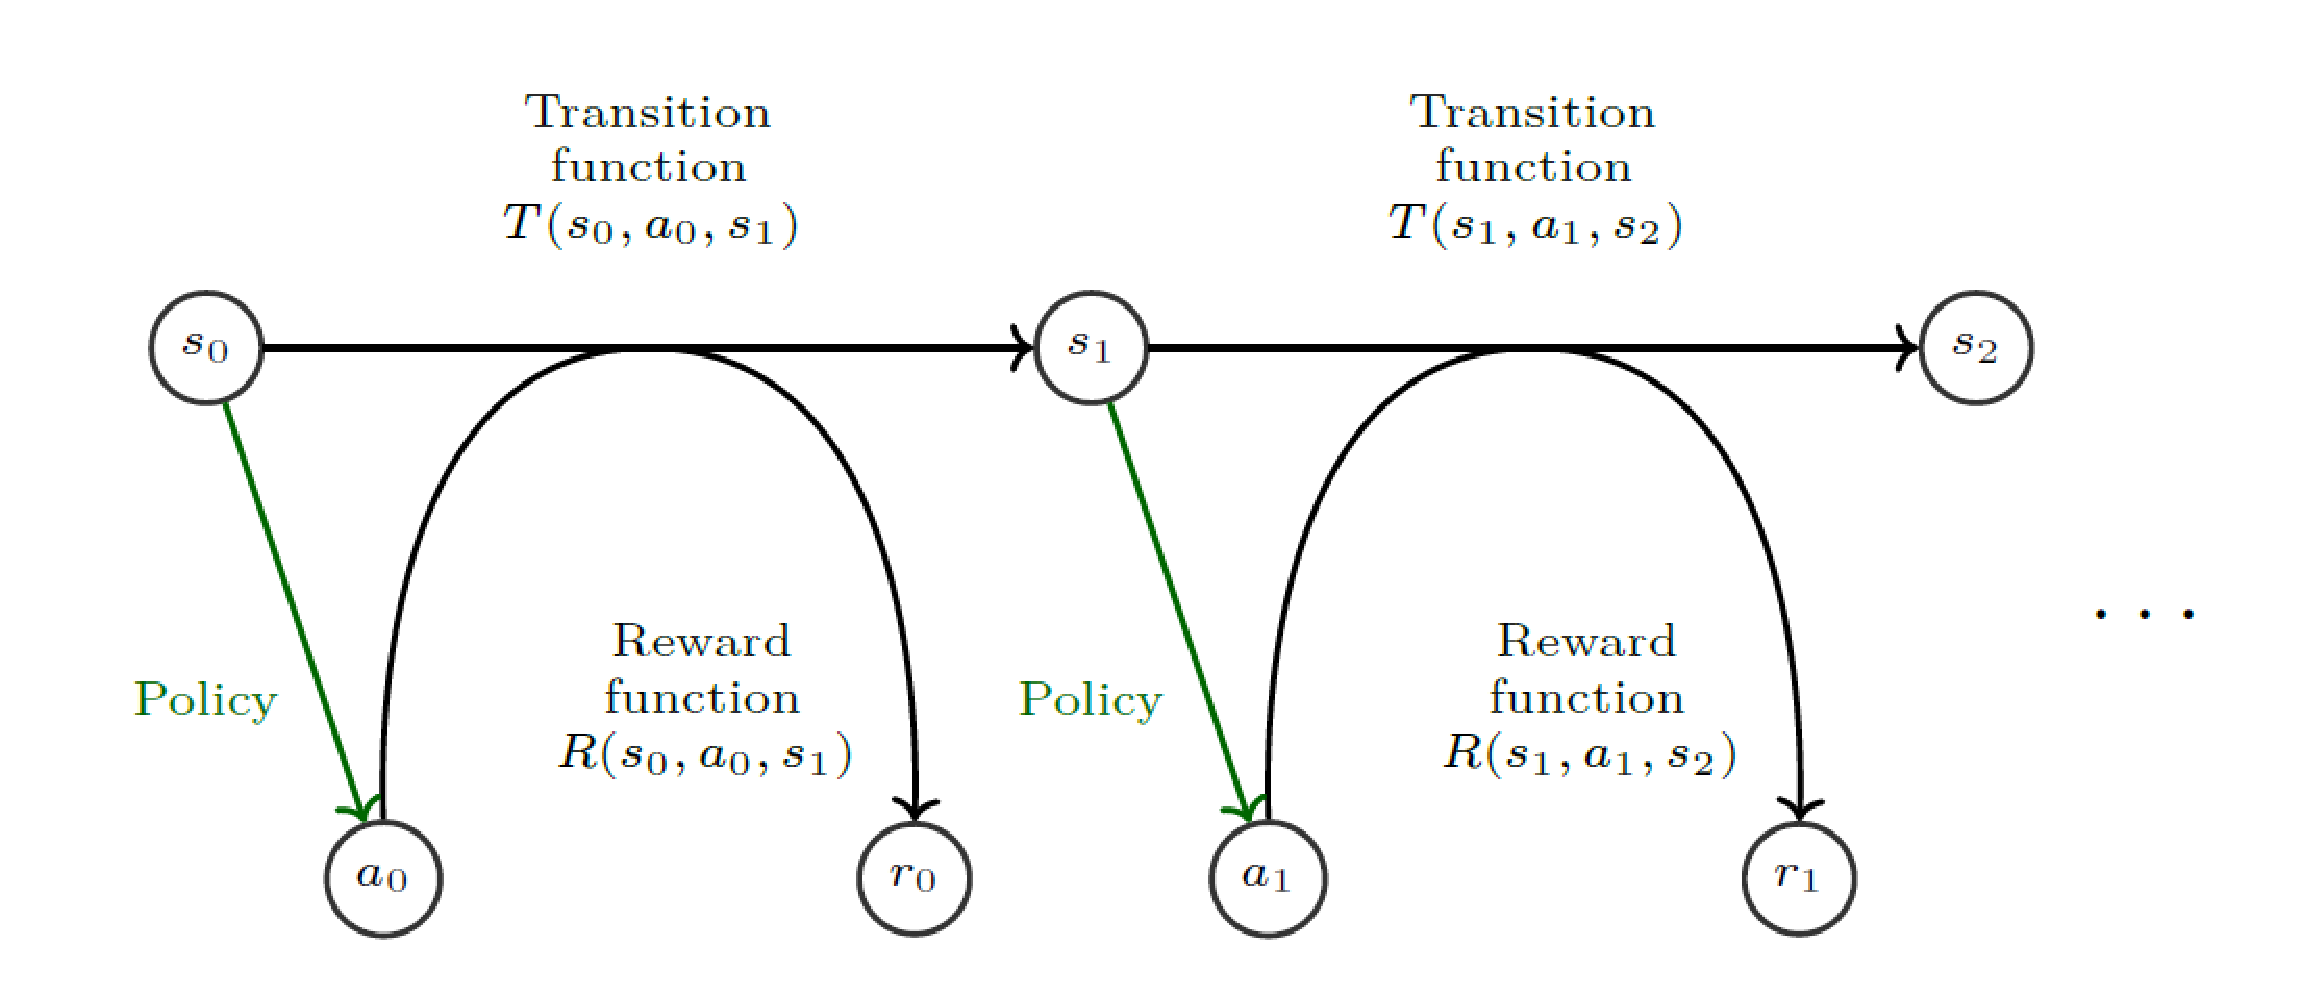
\includegraphics[width=.5\linewidth]{figs/mdp_detail.eps}
\caption{Agent takes an action to move to the next state and observe a reward \protect\cite{franccois2018introduction}} \label{fig:2}
\end{figure}

One of the most popular algorithms for learning optimal policies is Q-learning \cite{watkins1992q}. Q-learning is an off policy model free algorithm, which means that the agent does not learn transition and reward functions but instead learns so called Q-values from which the best possible action can be deduced. Each state in the state space has state-action pairs called Q-values. The Q-value $Q(s,a)$ describes the rewards an agent can expect from taking taking action $a$ in state $s$. For instance, if Mario encounters a Goomba in his current state, the Q-value for taking an action running into the Goomba would be lower than the Q-value for taking an action killing the Goomba. This is because the reward function returns negative rewards for dying at the hands of a Goomba and positive rewards for killing it. The optimal Q-value is described with the \textit{Bellman Optimality Equation} \cite{bellman1966dynamic}. It states that the Q-value of a state-action pair $(s,a)$ at timestep $t$ is the expected reward of that pair $R_{t+1}$ plus the maximum discounted return of the next state-action pair $Q(s^\prime, a^\prime)$:

%\begin{equation}
% Q^\pi(s, a) = \E \left[ \sum_{k=0}^{\infty} \gamma^k R_{t+k+1} \Big| S_t = s, A_t = a \right]
%\end{equation}

\begin{equation}\label{eq:optimal_q}
Q^*(s,a) = \E \left[ R_{t+1} + \gamma \max\limits_{a^\prime} Q(s^\prime, a^\prime) \right]
\end{equation}


Because an optimal policy will choose the action which returns the highest reward and Q-values tell us how much reward to expect from an action, an optimal policy chooses the action associated with the largest Q-value. Hence, to learn an optimal policy an agent needs to learn the Q function: $Q : S \times A \to \R$ of the problem. Learning the Q-function is a process of continuously experiencing the environment and using the observations to iteratively update the Q-values until they converge. Observations are the states and rewards associated with taking actions in the state space. The following equation shows the Q-value update:

\begin{equation} \label{eq:q_update}
	Q(s,a) \gets Q(s,a) + \alpha \left[ R + \gamma \max\limits_{a^\prime} Q(S^\prime, a^\prime) - Q(s,a) \right]
\end{equation}


Whenever an agent takes an action in a state and experiences a reward, the old Q-value needs to be updated to reflect that observation. This is done by adding the experienced reward $R$ for taking action $a$ in state $s$ to the discounted largest Q-value of the next state $Q(S^\prime, a^\prime)$ ($\gamma$ is the discount factor), subtracting the old Q-value, multiplying everything by the learning rate $\alpha$ and adding it to the old Q-value. The learning rate specifies the importance of new information \textit{vis-à-vis} old information. In traditional RL, the Q-function is a lookup table where each entry corresponds to a Q-value. Q-tables are suitable for low-dimensional problems with small state and action spaces, however they quickly become infeasible for complex problems. For instance, assuming an image size of $84 \times 84$, the RGB Super Mario state space has a size of $(84 \times 84 \times 3)^{256}$. Storing the Q-values for a state space of that size is impossible. The solution is to replace the lookup table with a neural network called a Deep Q-Network (DQN) or policy network. This is what turns traditional RL into Deep-RL. The preferred kind of network is a Convolutional Neural Networks (CNN). CNNs have become especially popular within the RL community because they facilitate end to end learning by identifying features in images and mapping them to outputs, thus removing the process of manually extracting features from game frames. Furthermore, CNNs reduce the need for a large memory footprint and allow for the application of RL to high-dimensional problems like video games. A video game Deep RL system usually has a \textit{policy network}. The policy network is a CNN that receives a game frame as input and outputs a vector of Q-values which can then be mapped to actions.

\begin{figure}[!htb]
\centering
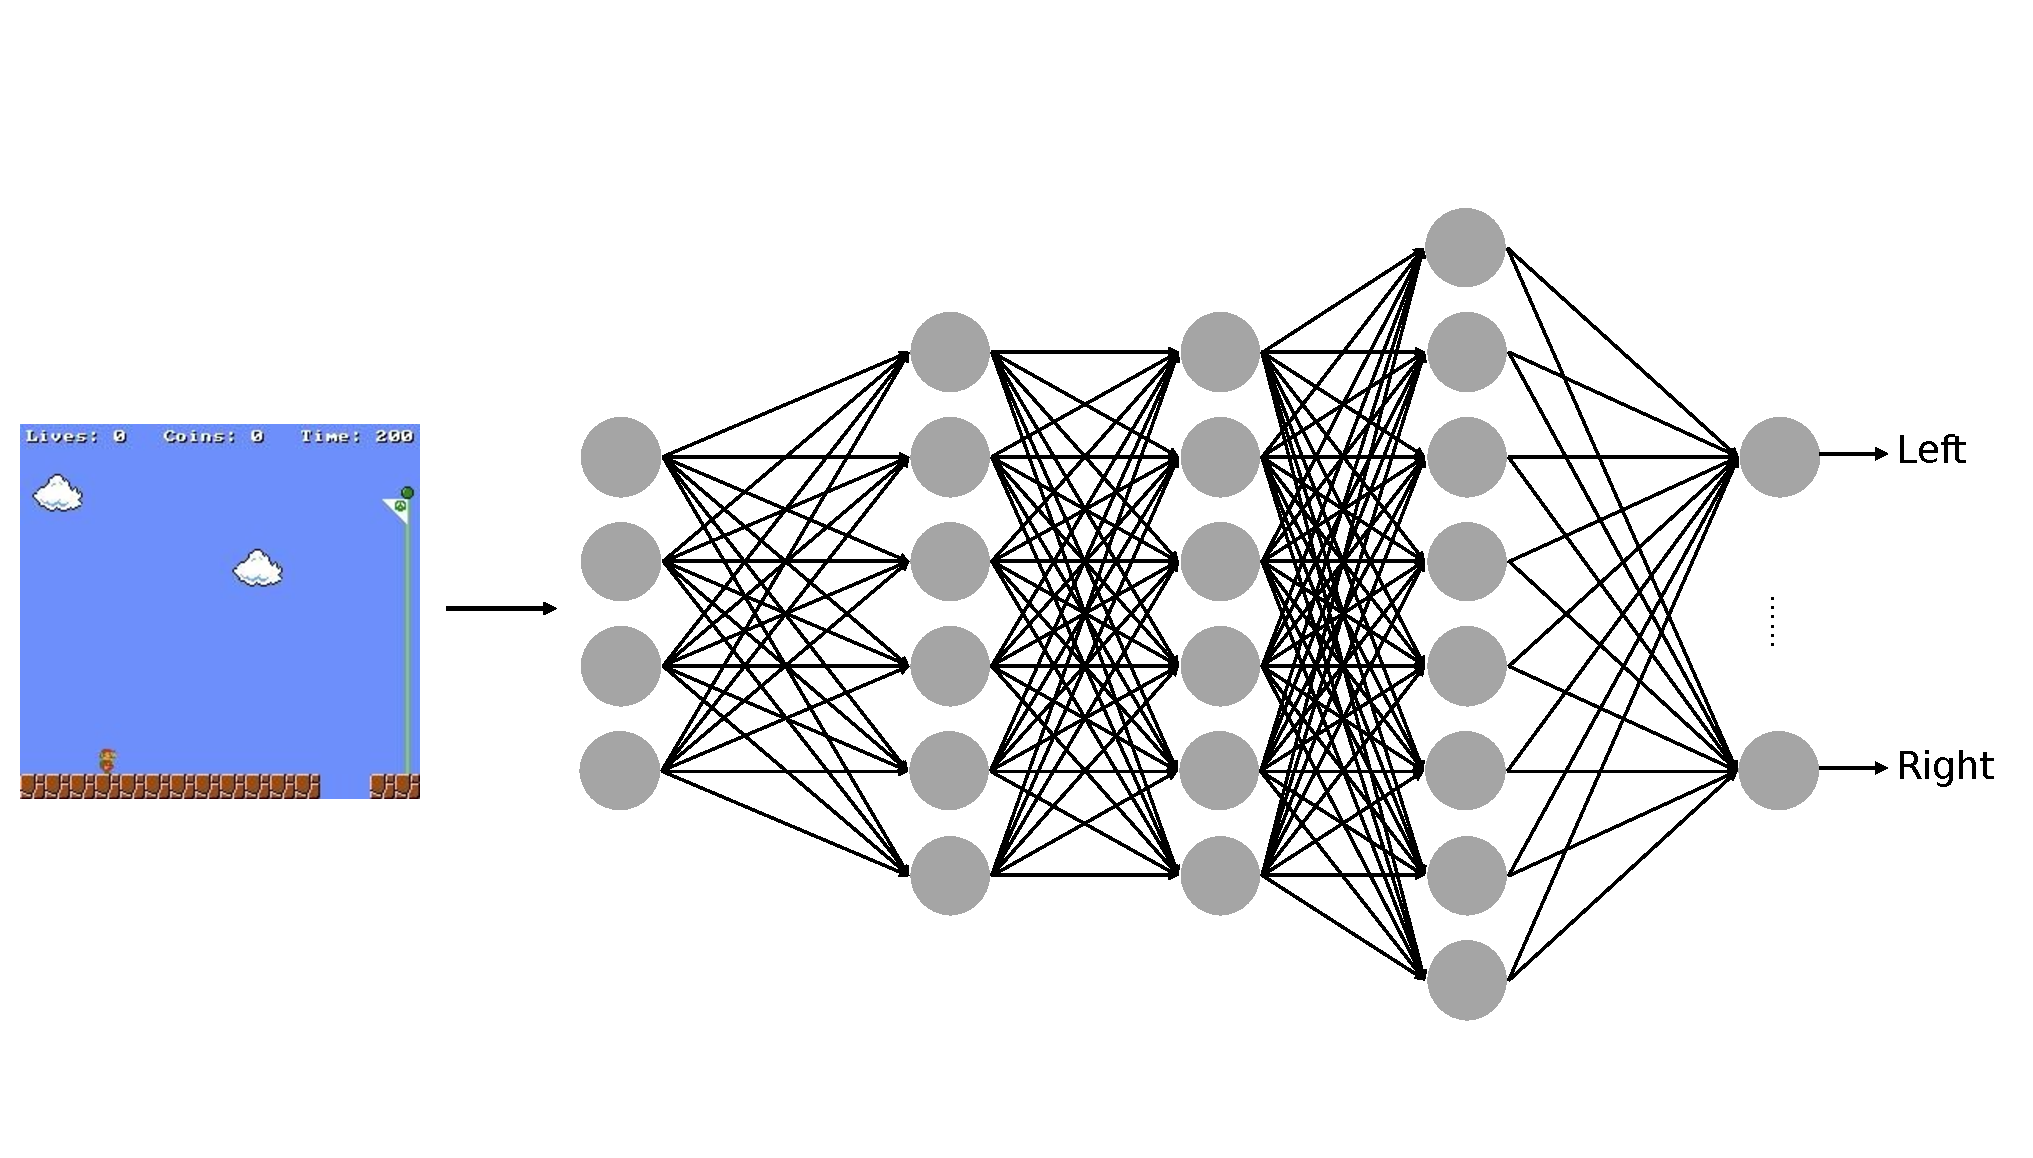
\includegraphics[trim={0 2cm 0 2cm},clip,width=.75\linewidth]{figs/deep_rl_video_game.eps}
\caption{Policy Network for Super Mario (not to scale)} \label{fig:2}
\end{figure}

The input first passes through a couple of convolutional layers designed to detect shapes and features such as edges and high level objects. Then follow fully connected layers to produce the output. For Super Mario, the state is represented as a pixel matrix of dimensions $(width \times height \times channels)$ where channels is the number of colour channels in the frame - 3 for RGB, 1 for grayscale. Given a state, the CNN performs a forward pass and outputs a vector of Q values. Because we want the most rewards possible and the Q-values tell the agent what rewards to expect, the agent choose the action associated with the highest Q-value. Having performed a forward pass, now all that remains is to train the network so that the agent can learn the optimal Q-values of the MDP. First, the loss of the network is calculated using a loss function such as the huber loss \cite{huber1992robust}, which is then differentiated with respect to the weights of the network before taking a gradient step. The network is fully trained when the output Q-values have sufficiently approximated the true Q-values of the MDP.  

\subsubsection{Target Networks}
The improvement made by replacing the Q-table with a neural network is significant, however an issue arises when calculating the network loss. The loss is computed as the difference between the outputted Q-values of the current state-action pair and the true Q-values. 

\begin{equation} \label{eq:q_loss}
	loss = Q^*(s,a) - Q(s,a) 
\end{equation}

Calculating the optimal Q-value of a state $Q(s,a)$ requires the maximum Q-value $Q(s^\prime, a^\prime)$ of the next state (see equation \ref{eq:optimal_q}). However, because the policy network is used to calculate both values, any weight updates to the network will shift both $Q(s,a)$ and $Q(s^\prime, a^\prime)$. At each iteration, $Q(s,a)$ will move closer to the optimal targeted Q-value. Yet the targeted $Q(s^\prime, a^\prime)$ will move as well and we end up chasing a moving target. Ultimately, this causes overestimation of the Q-values and leads to learning instabilities that result in poor policies. The solution is to use a separate target network with the frozen weights of the policy network to calculate the target Q-values. Therefore, target Q-values remain stationary when being approximated and the network does not overestimate Q-values. Periodically, the policy network's weights are copied to the target network so that they accurately reflect the learning process.


%\begin{figure}[!htb]
%\centering
%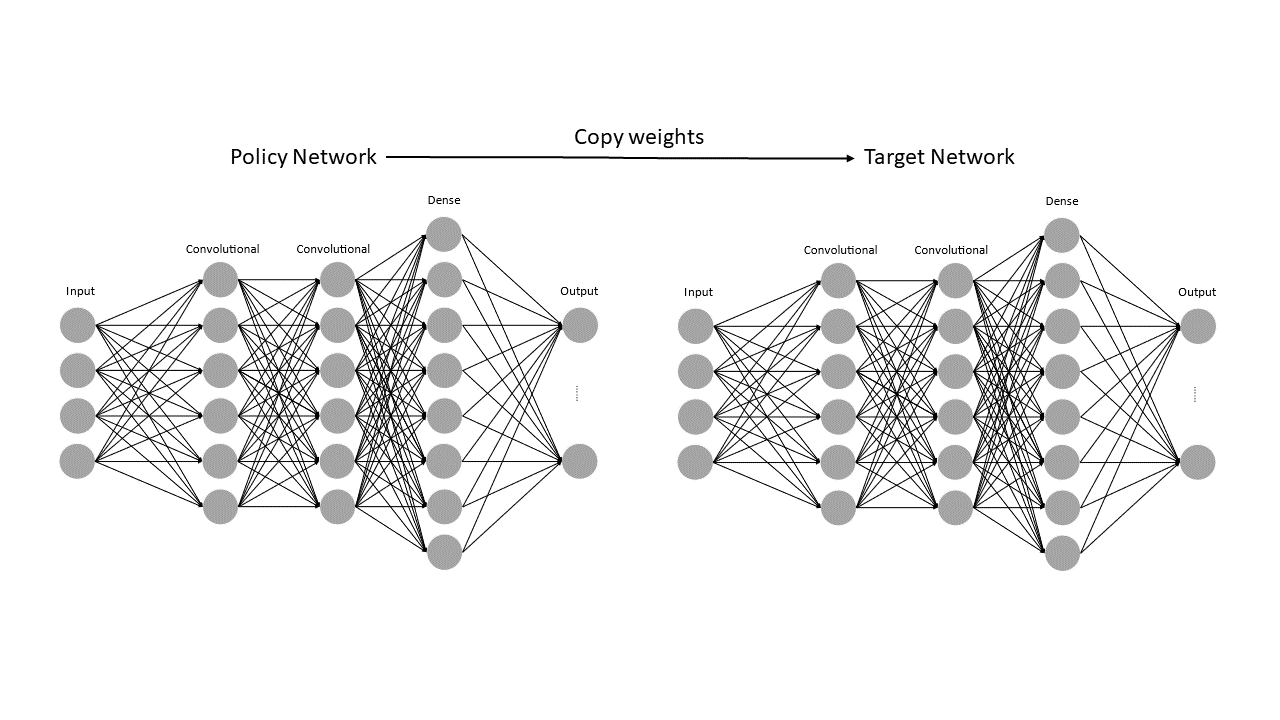
\includegraphics[trim={0 3cm 0 3cm},clip,width=1\linewidth]{figs/policy_target_nn.eps}
%\caption{Policy and Target Networks} \label{fig:2}
%\end{figure}

\subsubsection{Experience Replay}
In traditional RL, observations of the environment are immediately discarded after the Q-values have been updated. Experiencing the environment as a consecutive stream of temporally sequential observations becomes problematic because samples are highly correlated and training on correlated data may trap you in a local minimum. Furthermore, because observations are not kept, each one of them can only be used in a single weight update which makes learning less efficient. Therefore, most Deep Q Learning algorithms attempt to break correlation between samples and reuse them for weight updates with a \textit{replay memory} \cite{lin1993reinforcement}. The replay memory is a buffer of size $N$ where the agent stores experience tuples $e_t = (s_t, a_t, r_{t+1}, s_{t+1})$. The agent uses samples from the replay memory to train the DQN, not the live frame it currently sees. Until the agent has collected a sufficient number of samples, it will execute random actions. Once the memory has been filled with enough samples, the agent randomly samples a batch and uses it to train the policy network. 


\subsection{Hierarchical RL}
Arguably, one of humans' most remarkable abilities is the ability to generalise knowledge \cite{geirhos2018generalisation} across various contexts withstanding input distribution changes. For example, you are able to recognise a door as a door and open it regardless of its colour or material because you abstract away the features which make up the door and generalise those features to other doors. While Deep RL partially alleviates the issue of generalisation via its use of neural networks\cite{sutton1996generalization}, it remains a substantial issue \cite{van2017hybrid} to date. RL agents are prone to overspecialise and overfit because they are trained and tested within the same environment \cite{cobbe2018quantifying}. If Mario is trained to solve level \textit{World 1-1}, he only becomes an expert on that particular level. When placed in the next level, he would not perform as well because Mario did not \textbf{learn} any concepts of the world. Instead, he \textbf{remembers} optimal action sequences only applicable to a distinct problem. This is also known as \textit{flat} RL.

\begin{wrapfigure}{r}{0.5\textwidth}
	\vspace{-20pt}
	\begin{center}
		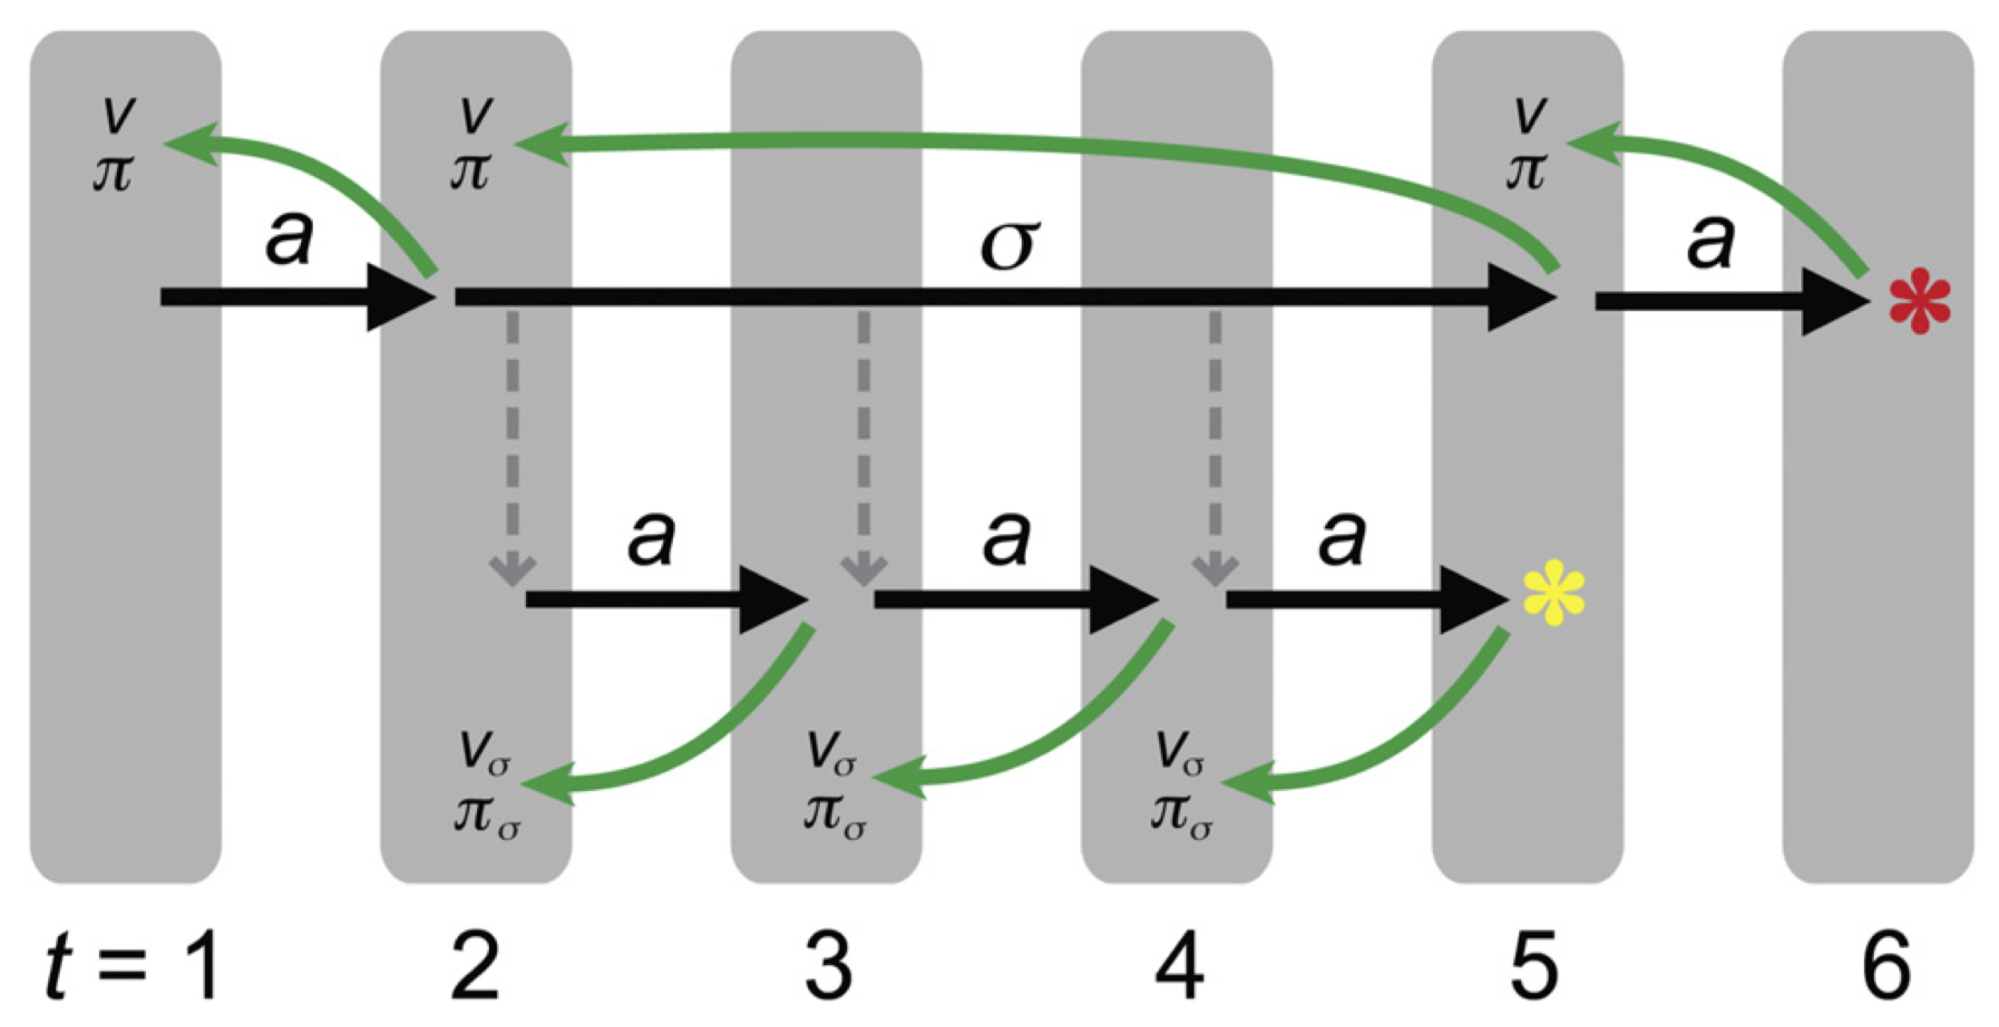
\includegraphics[width=0.4\textwidth]{figs/hrl_smdp.eps}
	\end{center}
	\vspace{-20pt}
\caption{The Hierarchical RL Semi Markov Decision Process \protect\cite{ribas2011neural}} \label{fig:hrl_mdp}
\end{wrapfigure}

Learning reusable skills is the essence of Hierarchical RL. It is inspired by the fact that human decision making is \textit{temporally abstract} \cite{sutton1999between} and hierarchically composed. When baking brownies, you need to follow a recipe composed as list of tasks which might include melting chocolate with butter, creaming eggs and sugar together before folding in flour and cocoa powder. Each of these can be considered as a subtask of the overall baking brownie task. Each action however can be further decomposed until we have reached a sequence of muscle contractions. A flat RL learning to bake brownies would only learn these muscle contractions whereas using Hierarchical RL the "melting butter with chocolate" and "creaming eggs with sugar" actions can be learned. And because these are not unique to baking brownies, they could be reused for making a chocolate cake as well. By decomposing the overall problem into smaller subproblems, learning is sped up and actions can be reused across the domain. This requires some modification to the MDP used in tradiational RL. In \textit{flat} learning, each action $a_t$ only lasts a single timestep. Now, the agent can execute actions lasting multiple timesteps. An action $a_t$ in state $s_t$ can transport the agent to state $s^{\prime}_{t+k}$. In Figure \ref{fig:hrl_mdp}, the policy $\pi$ is made up of multiple sub-policies, each of which are catering to a specific subset of the state space. At timestep $t_1$, the primitive action $a$ is selected and lasts one timestep. At $t_2$, the policy $\pi$ invokes a subpolicy or subtask $\sigma$ which is in charge of selecting primitive actions until $t_5$. Upon termination, the subpolicy returns a reward (yellow asterisk) back to the master policy which incorporates it into the value of the state from where the policy was invoked.

\subsubsection{Option-Critic}
The following Hierarchical algorithm builds upon the Markov-Options framework \cite{sutton1999between} which first introduced a framework for extending the classical one-timestep-action MDP to a multi-timestep-actions Semi MDP (SMDP). The SMDP contains \textit{Markov Options}, a layer of temporal abstraction on top of the primitive one-timestep actions of the agent. An option is defined as a triplet $\langle I, \pi, \beta \rangle$ where:

\begin{itemize}[noitemsep]
	\itemsep0em
	\item $I \subseteq S$ is the subset of states available to the option.
	\item $\pi : S \times A \to [0,1]$ is the policy for the option.
	\item $\beta : S^+ \to [0,1]$ is the termination criterion for the option.
\end{itemize}

An option can only be chosen by the agent if the current state is in the subset of states available to the option, $s_t \in I$. This restricts options to a specific portion of the state space. For every subsequent state reached in the option, it will terminate with probability $\beta(s_{t+k})$. In Sutton et. al's work, the options/subpolicies had to be handcrafted for the agent to learn and use them. Additionally, learning these subpolicies came at a great temporal and spatial expense because each option is solved as its own MDP. The Option-Critic architecture \cite{bacon2017option} improves upon this by not only discovering subpolicies autonomously, but also simultaneously learning the policy over options/master policy as well as subpolicies. The number of hierarchies is fixed at two. Furthermore, it assumes that options are available to the agent everywhere in the state space, which means that $I = S$. Just like vanilla Deep RL, Option-Critic utilises Deep Q Networks to approximate the Q value function so that the agent can find the Q-values associated with state-action pairs.



\begin{wrapfigure}{r}{0.5\textwidth}
	\vspace{-20pt}
	\begin{center}
		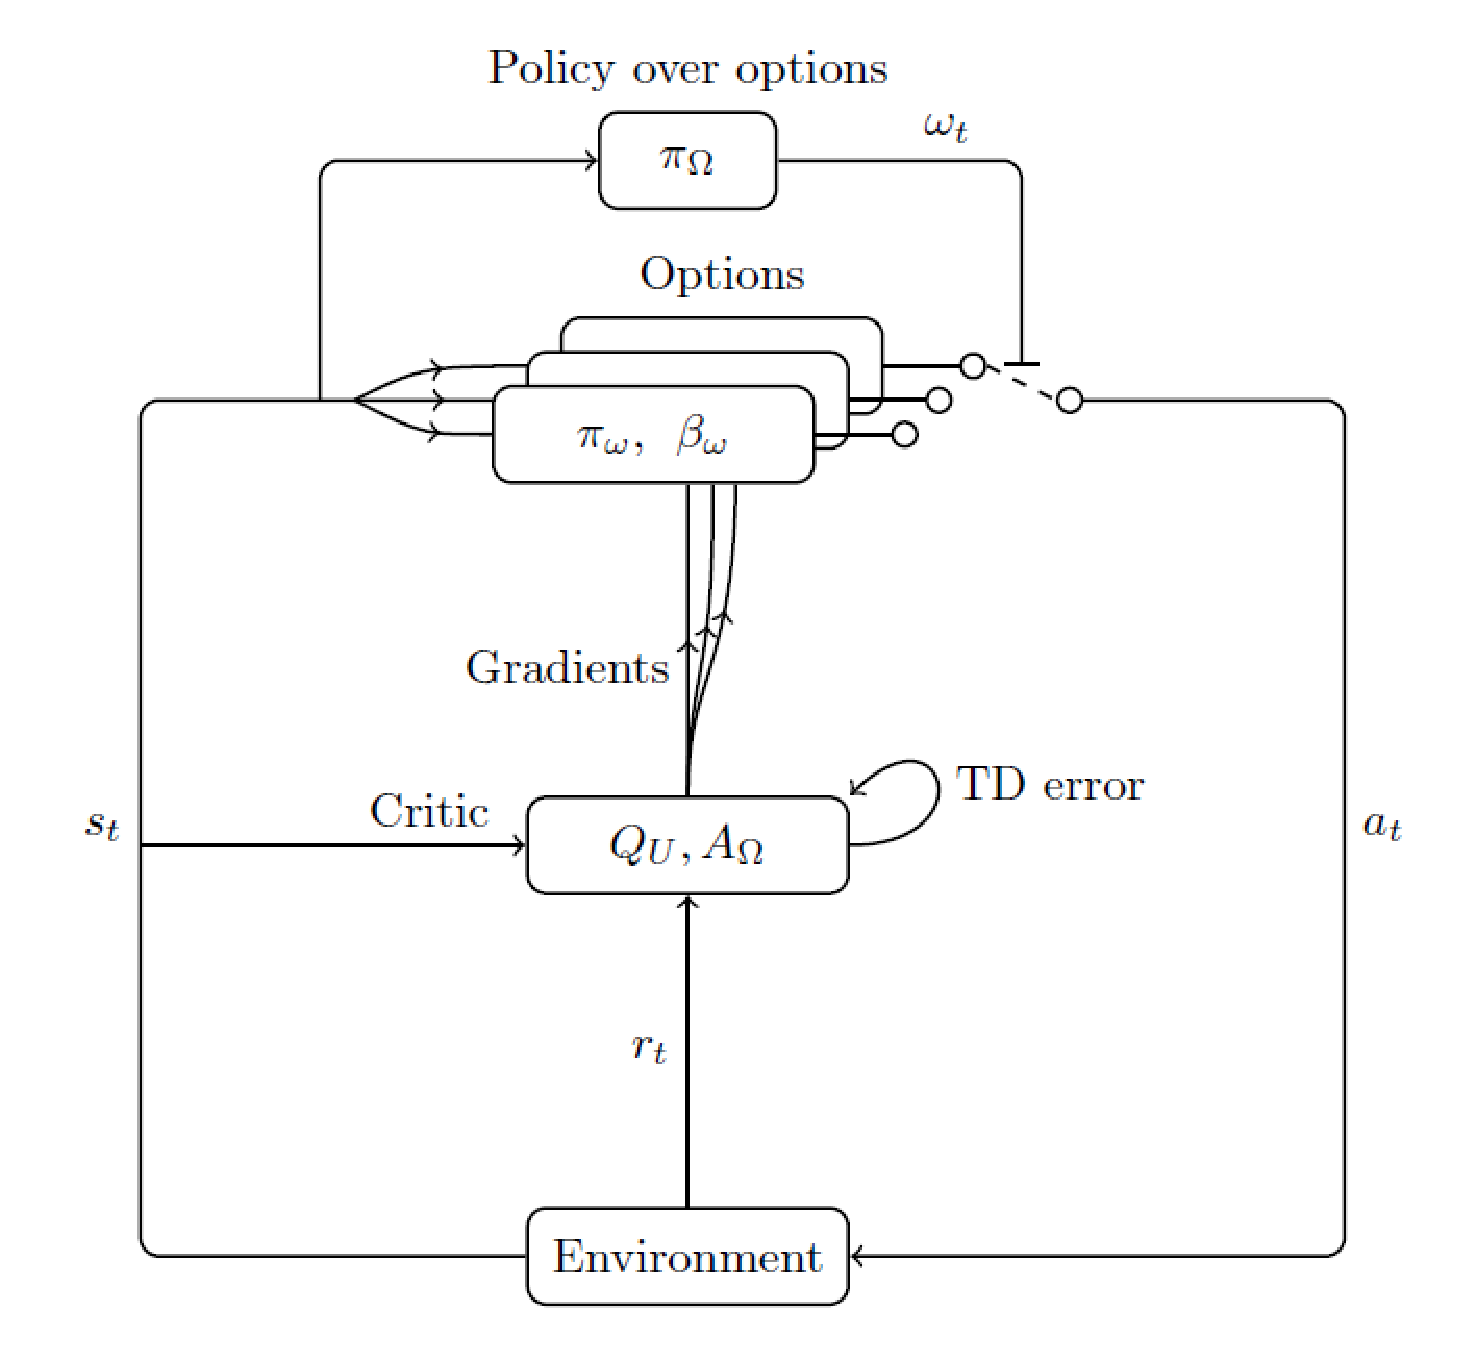
\includegraphics[width=0.4\textwidth]{figs/option_critic_architecture.eps}
	\end{center}
	\vspace{-20pt}
\caption{Option-Critic Architecture \protect\cite{ribas2011neural}} \label{fig:4}
\end{wrapfigure}

At each timestep, the master policy $\pi_\Omega$ chooses an option/subpolicy $\omega_t$. We follow the regular MDP structure where the option/subpolicy executes an action $a$ in the environment and receives a reward $r$ and new state $s^\prime$ in return. The critic then evaluates the option by using the Q-value $Q_U$, which is the reward estimate of executing the subpolicy $\omega$ from state $s$, to obtain the new Q update. If the next state is a terminal state of an option, we obtain the update value $\delta$ for the Q-value by subtracting the observed reward $r$ from $Q_U$. Otherwise, we compute the update value like we did for a terminal state and add the discounted Q-value $Q_\Omega$ of the entire option as well as the max Q-value of the \textbf{next} option. After evaluating, the option is improved using Stochastic Gradient Descent. The option terminates when the criterion $\beta_\omega$ is fulfilled after which the policy over options/master policy chooses the next option. The algorithm can be found in more detail in \textit{The Option-Critic Architecture} \cite{bacon2017option}.

\subsubsection{Feudal Networks (FuN)}
Another recent Hierarchical RL algorithm is DeepMind's FeUdal Network (FuN) \cite{vezhnevets2017feudal}. Like the Option-Critic architecture, is is an improvement on an older system, called Feudal RL \cite{dayan1993feudal}. Feudal RL follows the general Hierarchical RL architecture where different levels of temporal abstraction work together to solve the overall task. Taking after the questionable medieval feudal system, managers set goals for the sub-managers to solve in the state space and receive rewards once completed. Communication is restricted to a single vertical step in the hierarchy, meaning that each level can only give goals to the sub-manager below and receive goals from the manager above. Additionally, the number of hierarchies is theoretically unbounded. Though a great improvement on standard Q-learning, traditional Feudal RL is not general enough to work on multiple domains and has inherent convergence issues. DeepMind's FeUdal Network provides a fixed two-level manager-worker hierarchy encapsulating multiple neural networks. At the top is the manager, setting goals for the worker in the latent space. The latent space is a compressed version of the data. Working like a compass, the manager figures out \textbf{where} the worker should go. At the bottom, the worker has a high temporal resolution and is responsible for choosing primitive actions in the environment. Given a goal by the manager, the worker decides \textbf{how} to achieve it.

\begin{wrapfigure}{r}{0.5\textwidth}
	\begin{center}
		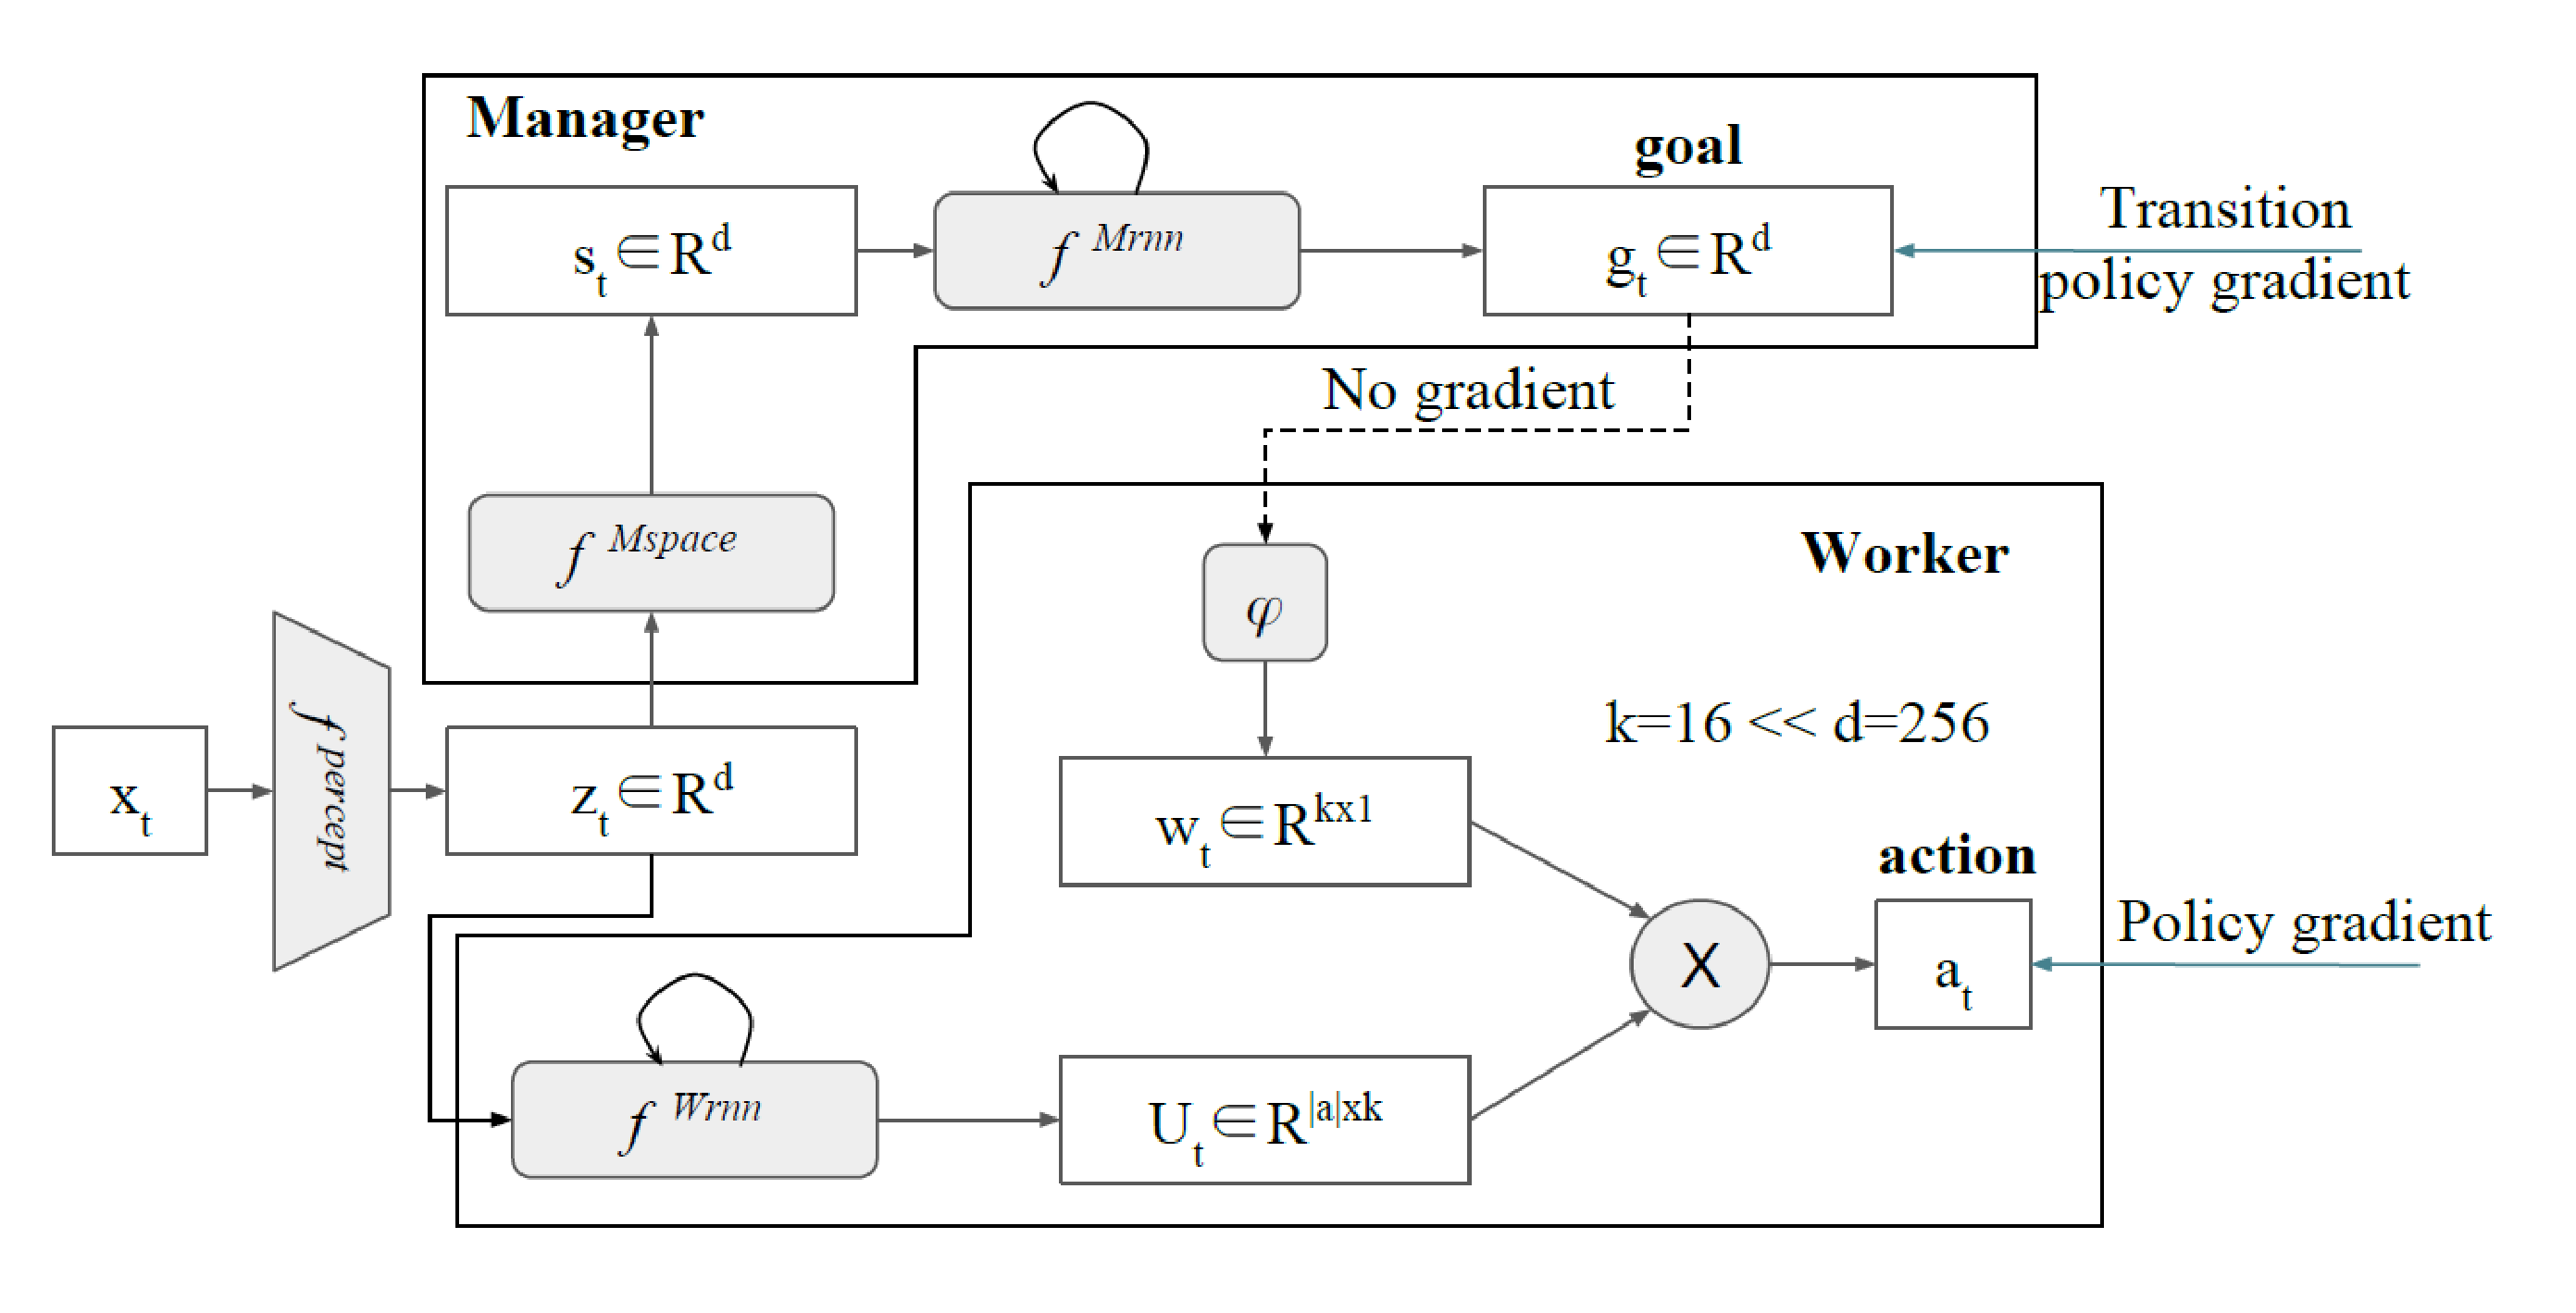
\includegraphics[width=.5\textwidth]{figs/fun_architecture.eps}
	\end{center}
	\caption{FuN Architecure \protect\cite{vezhnevets2017feudal}} \label{fig:4}
\end{wrapfigure}


FuN has a more complex architecture than the regular DQN and Option-Critic systems. First, the game frame is passed through a CNN modelled after DeepMind's Atari \cite{DBLP:journals/corr/MnihKSGAWR13} network to compute a separate intermediate representation $z_t$ of the state $x_t$ to be shared between the manager and worker. After further compressing the state $z_t$ into $s_t$, the manager utilises a Long short-term memory (LSTM) Recurrent Neural Network (RNN) to compute a goal $g_t$ for the worker to solve. The worker is given the intermediate state representation $z_t$ and uses an LSTM to produce an action embedding matrix $U$ where each row corresponds to a possible action within the game. To incorporate the manager's goal, the worker then embeds it into a vector $w_t$. By applying a dot product to the action matrix $U_t$ and the goal embedding $w_t$, we get a probability distribution over the actions which means that FuN produces a stochastic policy unlike the deterministic DQN and Option Critic. The FeUdal Network learns by a \textit{transition policy gradient} which boilds down to training the manager to predict goals which return large rewards in the state space. 

\section{System Requirements}

The following section specifies the requirements to be fulfilled by the system:

\begin{itemize}

	\item \textbf{Super Mario Game Emulator}\\ 
	The RL agent within the system must have the ability to interact with the Super Mario Bros game environment to obtain information about states, rewards and to perform actions. The Python OpenAI Gym library provides a plugin to play Super Mario, however this plugin does not allow the creation of custom levels (more on custom levels in the next point). Instead, the sytem will use the Mario AI Tenth Anniversary Edition \cite{marioai} framework. Although written in Java, it provides the user with the ability to create their own levels using ASCII art.
	
	\item \textbf{Custom Levels}\\
	Using custom levels means that we can better investigate Mario's generalisation abilities. The agent can learn specific skills in specially designed levels and slowly expand their skillset. This is also the main reason for choosing the Mario AI Tenth Anniversary Edition framework over the OpenAI Gym library. OpenAI Gym only provides the original Super Mario levels and therefore makes the skill stacking with Hierarchical RL algorithms less transparent.
	
	\item \textbf{Reward Function}\\
Every MDP has a reward function. Because the chosen Super Mario framework does not have a reward function, it will first need to be designed. The function should incentivise the intended behaviour of the agent - to move as far right as possible in the level without dying.
	
	\item \textbf{Java-Python Bridge}\\
	Because the Super Mario game framework is written in Java and Python is the de facto lingua franca of RL, the system needs to have a communication bridge between the languages. The system needs to train for longer periods of time, so avoiding unnecessary overhead whereever possible is important. Getting the two languages "as close" as possible to each other is therefore vital. A client-server architecture using HTTP to send JSON is easy to implement, however comes with too much overhead. The Jython \cite{jython} and JPype \cite{jpype} frameworks allow for Python code to be executed in a Java environment by being directly embedded in the JVM. This reduces latency, however they have a steep learning curve and in the case of Jython only support Python 2.7. The Py4J \cite{py4j} framework on the other hand uses sockets to communicate with the Java API which leads to a slight performance decrease. Though it is nearly effortless to setup and easy to use which is why it is the best choice for the system.
	
	\item \textbf{Deep Learning Libraries}\\
	Contemporary RL algorithms rely on Neural Networks to learn behaviour. The system needs to be able to initialise and train neural networks by making use of existing libraries. PyTorch is the most suitable option as it offers a good balance between low-level granularity and easy to use high-level API. Additionally, PyTorch has their own RL tutorials.
	
	\item \textbf{Python Game Interface}\\
	The different RL agents of this project all need to interact with the Super Mario Java game emulator. Writing a Python interface that bridges to the emulator and provides standard operations for the agents to use will reduce code duplication on the agents' part and decouple them from the emulator logic.
	
	\item \textbf{Preprocessing}\\
	The environment as observed by the RL agent is a pixel matrix of the current frame of the game. Commonly, frames are cropped and scaled before being passed to the neural network. Cropping removes unnecessary information such as the score and timer counters at the top of the screen. Scaling reduces the complexity of the image and the number of neurons needed in the network. To reduce latency, cropping and scaling will need to be done on the Java side of the system.
	
	\item \textbf{Monitor Training}\\
	RL algorithms need to train for periods lasting from several hours to several days. Monitoring this process while it is going on is important because bugs can be caught early on and hyperparameters are more easily compared. Tensorboard provides tools for visualising various metrics such as rewards and loss. Graphs are updated live as the training is happening and the data can be downloaded as JSON or CSV for further analysis.
	
	\item \textbf{Remote Training}\\
	The entire system needs to be able to run locally as well as remotely in the cloud. Hardware in the cloud is more powerful and can be scaled up and down as needed. Additionally, it is robust against failures and accidents. Google Cloud provides APIs specifically designed for Machine Learning and comes with free credits for first time users.
	
\end{itemize}

	

\section{System Implementation}
The following section will describe the system architecture in detail as it was implemented from the requirements section.


\subsection{Overall Architecture}
The system follows a client-server model where the RL client uses the Py4J bridge to execute actions on the game emulator server and observes states and rewards in return. The client first initiates the environment via the game interface and receives back the start state of the MDP (note that this process is not displayed in the game server diagram in Figure \ref{fig:system_architecture}). Having chosen an action according to their policy, the agent passes a \textit{tensor} with said action to the game interface which encodes it as a \textit{boolean action vector}, e.g. $\begin{bmatrix} false & true & false & true & false\end{bmatrix}$. When the action vector is received by the Game Server via Py4J, the action is executed in the environment $k$ times (see section \ref{frame_stacking_skipping} for frame skipping). Having executed the acition $k$ times, the final frame of the action sequence is cropped and resized (see section \ref{frame_preprocessing}) and the reward is calculated using the environment's reward function (see section \ref{reward_function}). The reward and the frame are then marshalled back to the client using Py4J and extracted by the RL Agent using the game interface. At every timestep and after every completed episode, the agent writes the observed reward and the calculated loss into tensorboard. Once training has finished, the models and hyperparameters are saved for demonstration, evaluation and further training.

\begin{figure}[!htb]\label{fig:system_architecture}
\centering
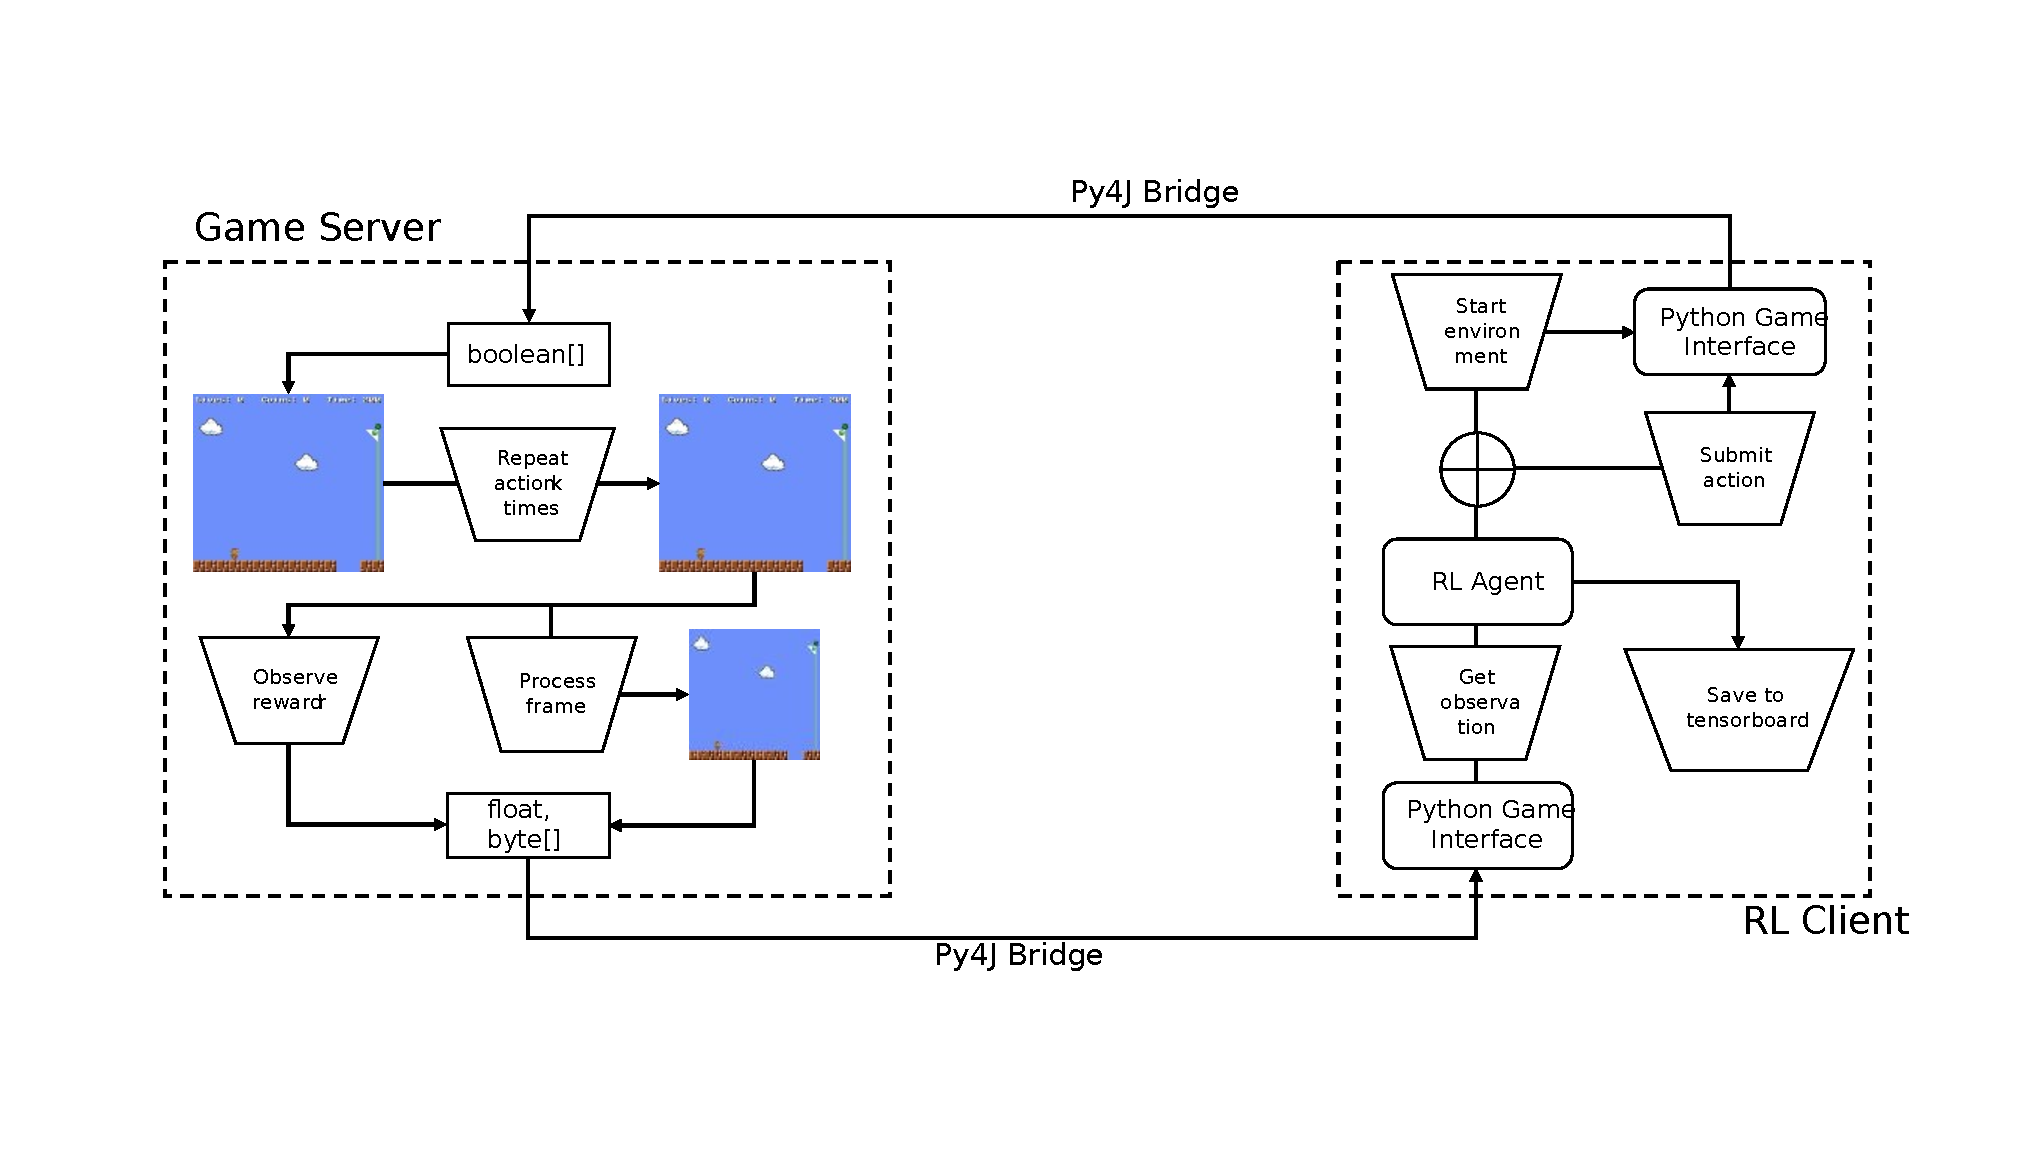
\includegraphics[trim={0 2cm 0 2cm},clip,width=.75\linewidth]{figs/system_architecture.eps}
\caption{System Architecture}
\end{figure}

The game server is a \textit{jar} file built using \textit{maven} exposing a port for the client to interact with. It is based on the \textit{marioai} \cite{marioai} framework which had to be . extended and rewritten to fit the requirements of the system. Various methods and classes for calculating the reward, preprocessing the game frame and exposing the observations of the environment to an outside agent were added to the existing codebase. To allow for remote training, both client and server are running on a single 4CPU 16GB Google Cloud virtual machine. Although only relying on CPU power to the run the system is prolonging training times, the expense of adding GPUs was considered too much for this project.


\subsection{Reward Function} \label{reward_function}

A RL agent learns to distinguish between desirable and undesirable behaviour by observing the reward signal associated with actions in the environment. At each time step $t$, the agent receives a scalar reward $R_t \in \R$ as a result of an action taken at time step $t-1$. The agents goal is to maximise the total reward it receives $\sum^{t}_{i=1} R_i$. The agent needs to receive rewards such that when maximised achieve the goal or solve the problem that we set out. It is important to note that the reward tells the agent \textit{what} it should achieve but not \textit{how} it should be achieved. Designing a reward function improperly might lead to unintended and unwanted behaviour, also known as the \textit{cobra effect}\cite{siebert2001kobra}.It is important to remember that in the end, you always get the behaviour you incentivised, not always the behaviour you intended. A well-crafted reward function aligns the \textbf{incentivised} behaviour with the \textbf{intended} behaviour.

%During British colonial rule in India, the government offered a reward for dead cobras as a way to reduce their population. Eventually, people began breeding cobras for income to milk the system and the program was scrapped. Breeders then set their snakes free, leading to an increase in the cobra population \cite{siebert2001kobra}. This is a pertinent example of how a flawed reward function can produce unwanted behaviour. 

Luckily, simple video games such as Super Mario often have clear criteria for success and failure, meaning that reward function design is of relatively low complexity. We want to incentivise Mario to reach the flag at the end of the level (success) and avoid anything that results in death (failure). Giving Mario positive rewards for moving right in the level and negative rewards for moving left forces Mario to keep moving right. Additionally, providing large negative rewards in terminal failure states and large positive rewards in terminal success states further forces Mario to stay alive and move towards the flag. Positive rewards encourage the agent to keep playing and accumulating those rewards. However, an agent may potentially avoid a terminal state to keep racking up rewards, known as \textit{reward hacking} \cite{amodei2016concrete}. Therefore, it is important to have positive terminal state values which make the agent choose the terminal state over reward hacking. Negative rewards on the other hand encourage the agent to finish the level as quickly as possible because they are constantly losing points. With this in mind, besides death, the agent is also penalised each time step $t$ to avoid him standing still. Thus, the agent will want to reach a terminal state as quickly as possible.
\linebreak
The reward function used in this project is inspired by the  \textit{openai gym} Super Mario Bros framework \cite{pypi}. It is composed of three variables $v, c, d$:

\begin{itemize}

	\item Velocity: $v = x_t - x_{t-1}$. The difference in the agent's \textit{x} values in between time steps $t$ and $t - 1$. Moving right will increase $v$.
	
	\item Clock: $c = c_t - c_{t-1}$. The difference in the game's clock values in between time steps $t$ and $t - 1$. For each action committed in game, $c$ will decrease by $1$. This is to prevent the agent from standing still.
	
	\item Death/Win: 
		\begin{equation*}
   	 		d = \begin{cases}
               			100               & \text{Mario wins}\\
               			-100              & \text{Mario dies}\\
               			-100				 & \text{Game times out}\\
           			\end{cases}
		\end{equation*}
		
		The death and timeout penalty encourage to avoid death and finish the level as quickly as possible. The win reward is to provide an extra incentive to visit the winning terminal state. In the original game, Mario receives more points the higher up he hits the flag at the end of the level. This was not modelled in the reward function to reduce its complexity.
		
	\item The reward function $r$ is the summation of the three variables $r(v, c, d) = v + c + d$. Additionally it is clipped in the range of $(-100, 100)$.
	
	
\end{itemize}


\subsection{Exploitation vs Exploration}\label{exploit_explore}
A major challenge within RL is to strike a balance between gathering enough information about the environment (exploration) and obtaining as much reward as possible (exploitation) \cite{sutton2011reinforcement}. A greedy agent will choose the action which according to their current knowledge returns the largest reward - \textit{exploitation}. Though for an agent to exploit an action they must previously have explored it enough times to have a reliable estimate on the action's reward. Being greedy produces large short term rewards, however the agent might ignore other options with potentially even larger rewards. Performing exploration could uncover those options and therefore lead to more reward in the long run. The dilemma arises when at each time step, the agent must decide whether to exploit or explore the environment. Exploring too much makes the agent a slow but steady learner. Exploiting too much means that the agent will quickly converge on their choice of actions but ultimately not act optimally.

\begin{wrapfigure}{r}{0.5\textwidth}
\vspace{-40pt}
  \begin{center}
    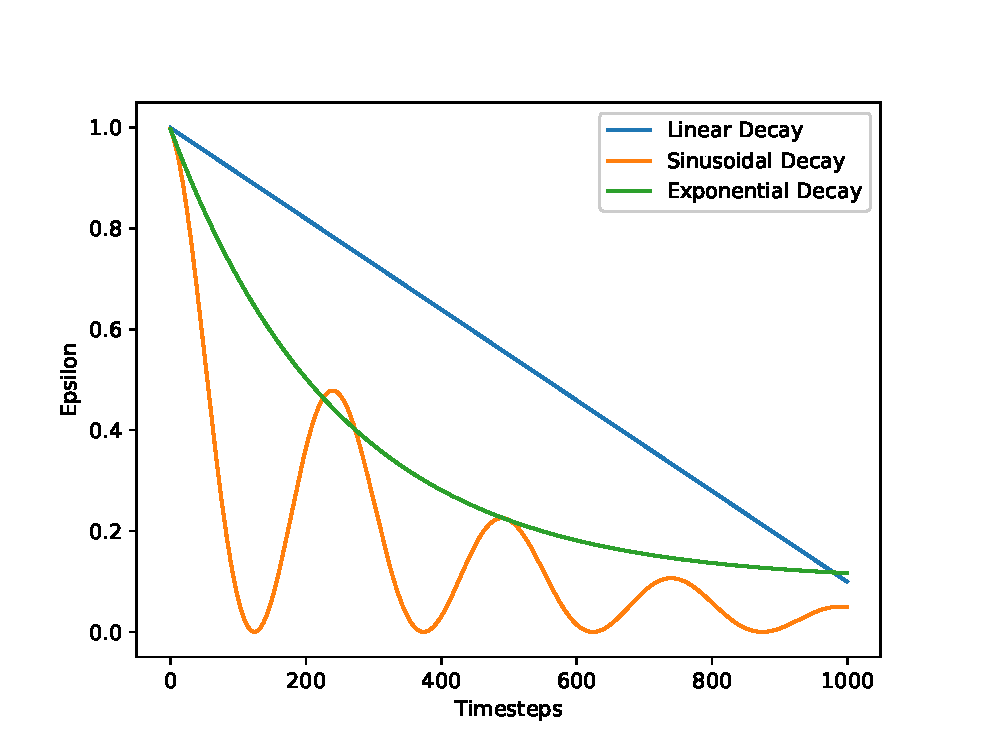
\includegraphics[width=0.48\textwidth]{figs/epsilon_decay.eps}
  \end{center}
  \vspace{-20pt}
  \caption{Variations of $\epsilon$ Decay}
  %\vspace{-40pt}
\end{wrapfigure}

A popular policy for choosing between exploitation and exploration is the $\epsilon$-greedy algorithm \cite{white2012bandit}. At each timestep, the agent chooses the best action to exploit the environment with $1-\epsilon$ probability. Exploration is more desirable at the beginning of the learning process because the agent does not possess enough information about the environment yet. Hence, the value for $\epsilon$ is usually decayed over time to reflect this. Methods for decaying $\epsilon$ can be linear \cite{mnih2015human}, exponential \cite{maroti2019rbed} and sinusoidal  \cite{chuchro2017game}. The algorithms that use an $\epsilon-Greedy$ policy in this project use a linear decay.


\subsection{Frame Preprocessing} \label{frame_preprocessing}
Preprocessing data is a step all Machine Learning systems go through prior to starting the actual learning. For a RL network, the input is a pixel matrix representing a game frame. For Super Mario, the dimensions of the raw image as returned by the game are $240 \times 256 \times 3$. Before the raw image can be passed to the network, it needs to go through a series of preprocessing steps aimed at reducing its dimensionality to make learning less computationally demanding. First, unnecessary information such as the score, lives, and timer and cropped out because they do not provide relevant clues to the agent. Second, the image is resized to $84 \times 84 \times 3$ using bilinear interpolation \cite{gribbon2004novel} to reduce the size of the neural network needed for training. The dimensions $84 \times 84$ are taken from DeepMind's \textit{Playing Atari with RL} paper \cite{DBLP:journals/corr/MnihKSGAWR13}. Converting the image to grayscale is often applied preprocessing step, though grayscale models tend to perform lower \cite{lample2017playing}.

\begin{figure}[!htb]
\centering
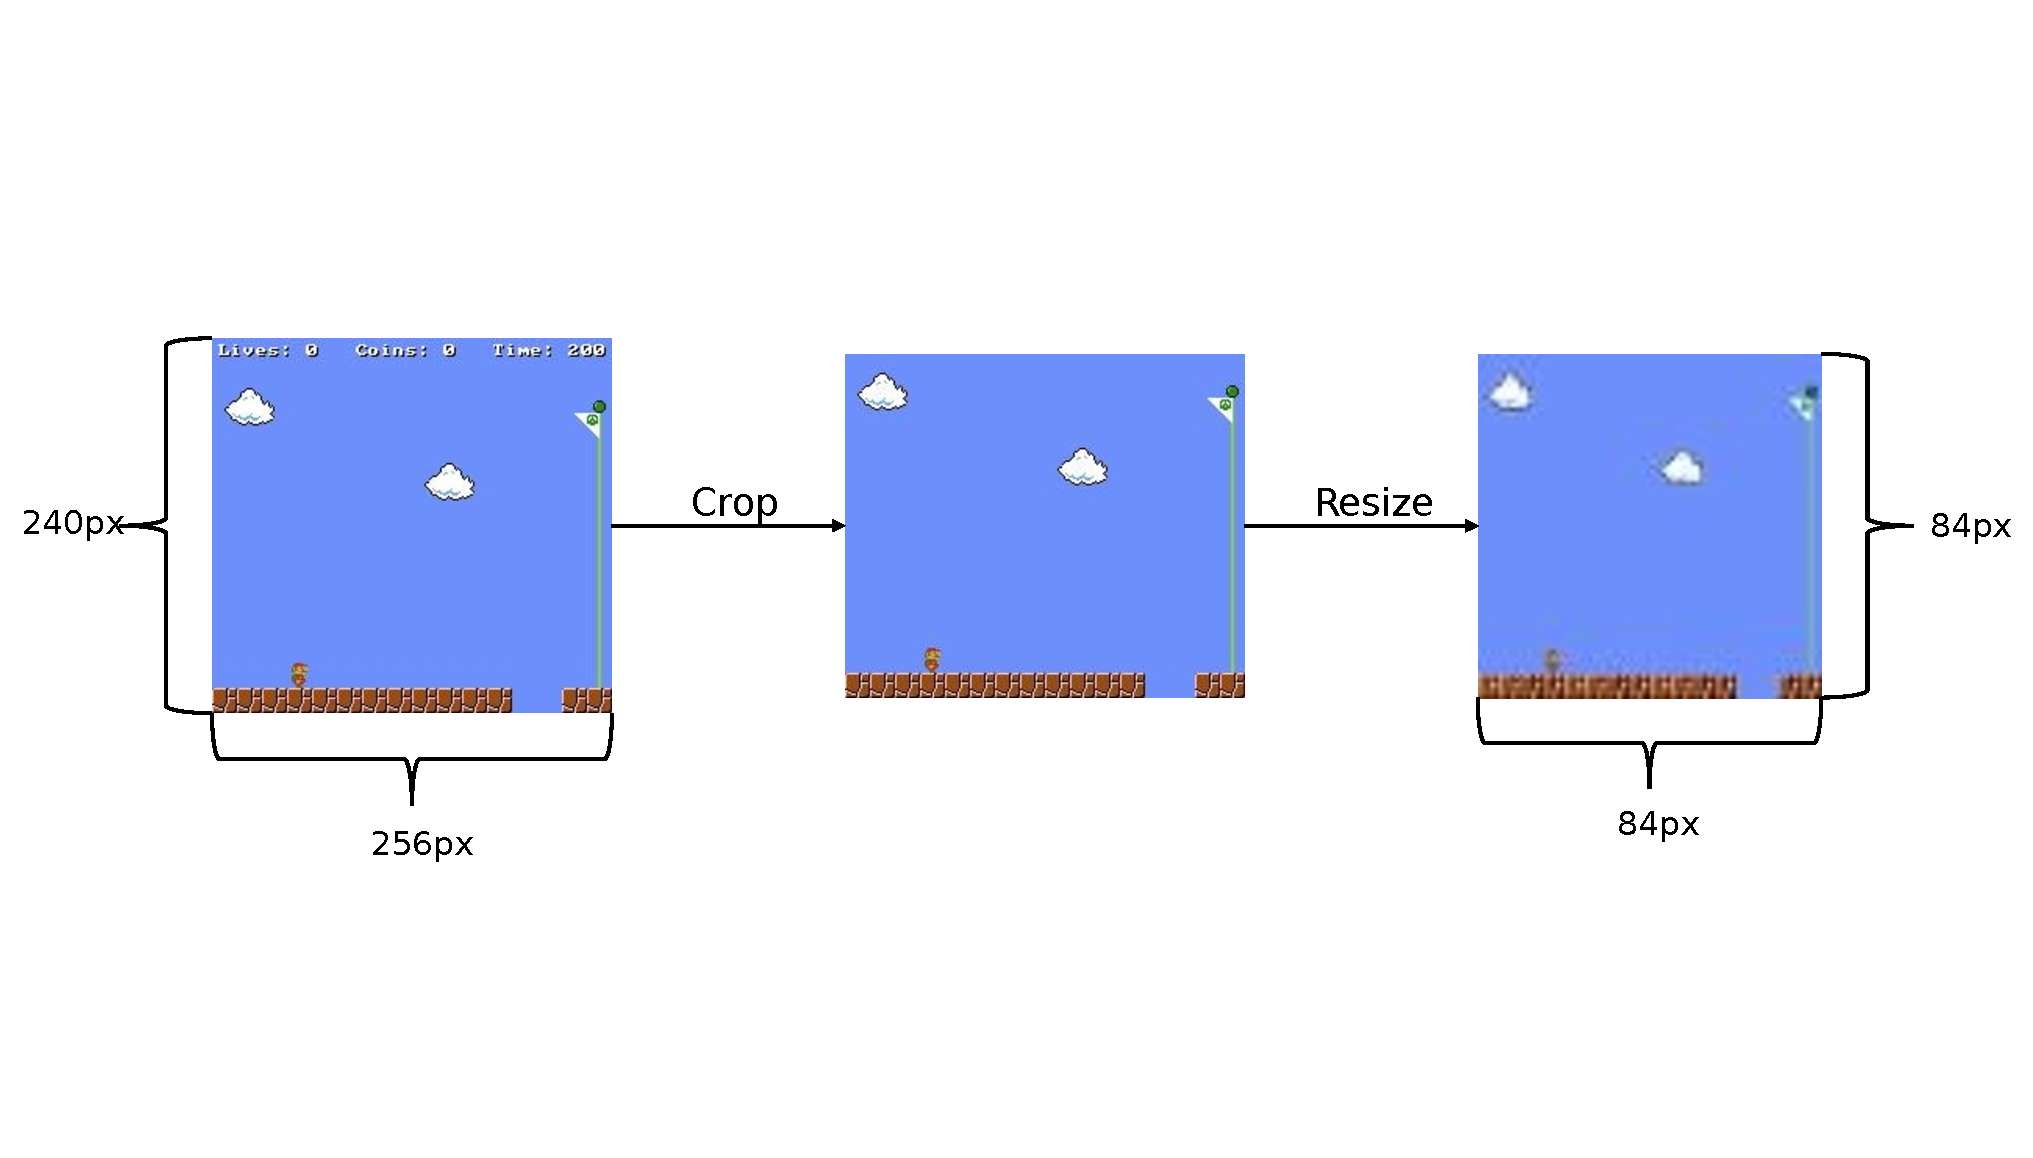
\includegraphics[trim={0 4.5cm 0 5cm},clip,width=1\linewidth]{figs/frame_preprocessing.eps}
\caption{Frame Preprocessing Pipeline}
\end{figure}



\subsection{Frame Stacking and Frame Skipping} \label{frame_stacking_skipping}
When playing a video game, it is important for the player to have a sense of how the objects in the environment are moving. Looking at a single frame of Super Mario does not tell you whether Mario is moving left, right, up or down. Only when presented with consecutive frames could you actually determine Mario's movement. Hence, to give the policy network of our system an idea of where Mario is going, it is fed a stack of 4 frames as input during training. Using 4 frames was again pioneered by DeepMind \cite{DBLP:journals/corr/MnihKSGAWR13}.

\begin{figure}[!htb]
\centering
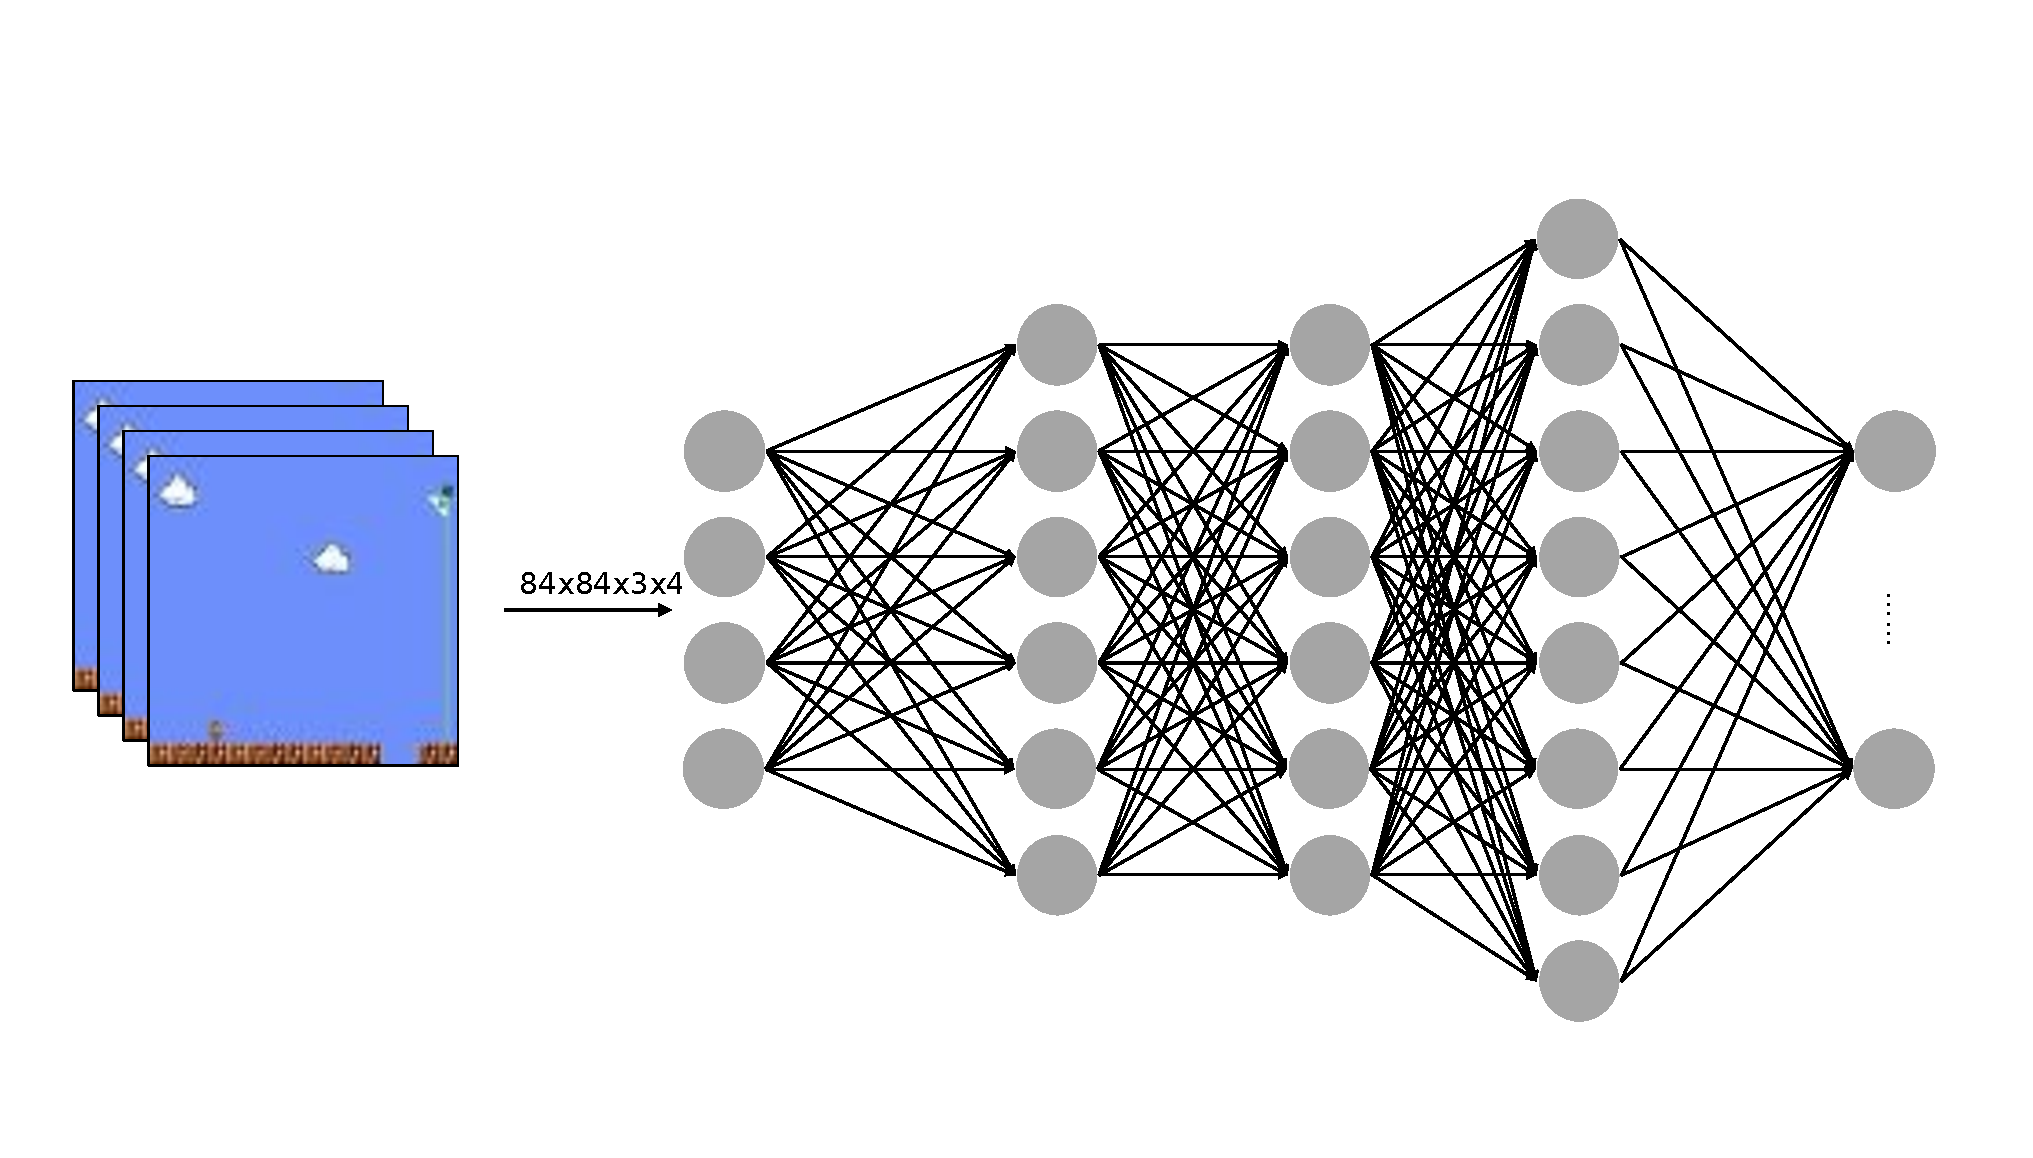
\includegraphics[trim={0 2cm 0 2cm}, clip, width=.75\linewidth]{figs/frame_stacking_nn.eps}
\caption{Stacked frames are given as input to the neural network. The dimension of the input thus becomes $84 \times 84 \times 3 \times 4$}.
\end{figure}

Another trick DeepMind used in their paper is to only show the agent every $k^{th}$ frame of the game. Instead of taking an action for every frame in the game, the agent now decides on an action every $k^{th}$ frame. The chosen action is then repeated for $k$ frames. This idea is partially motivated by how humans would play the game. A human player makes decisions on how to proceed in the game not for every frame they observe, but at intervals depending on the game environment (some games require faster reactions than others). Using frame-skipping also has the benefit of speedier learning because executing actions in the emulator is faster than doing a forward pass through the policy network to decide on an action. Choosing a value for $k$, one must factor in the desired resolution granularity. A large value for $k$ means that episodes can be played faster because the emulator is doing more work than the policy network. However, the agent might miss out on opportunities in the game because the same action is repeated too many times \cite{braylan2015frame}. On the other hand, agents may learn associations between temporally distant states and actions when skipping a large amount of frames. A small $k$ gives the agent finer granularity, though at the cost of longer episodes. This project uses the value $k = 4$.

\begin{figure}[!htb]
\centering
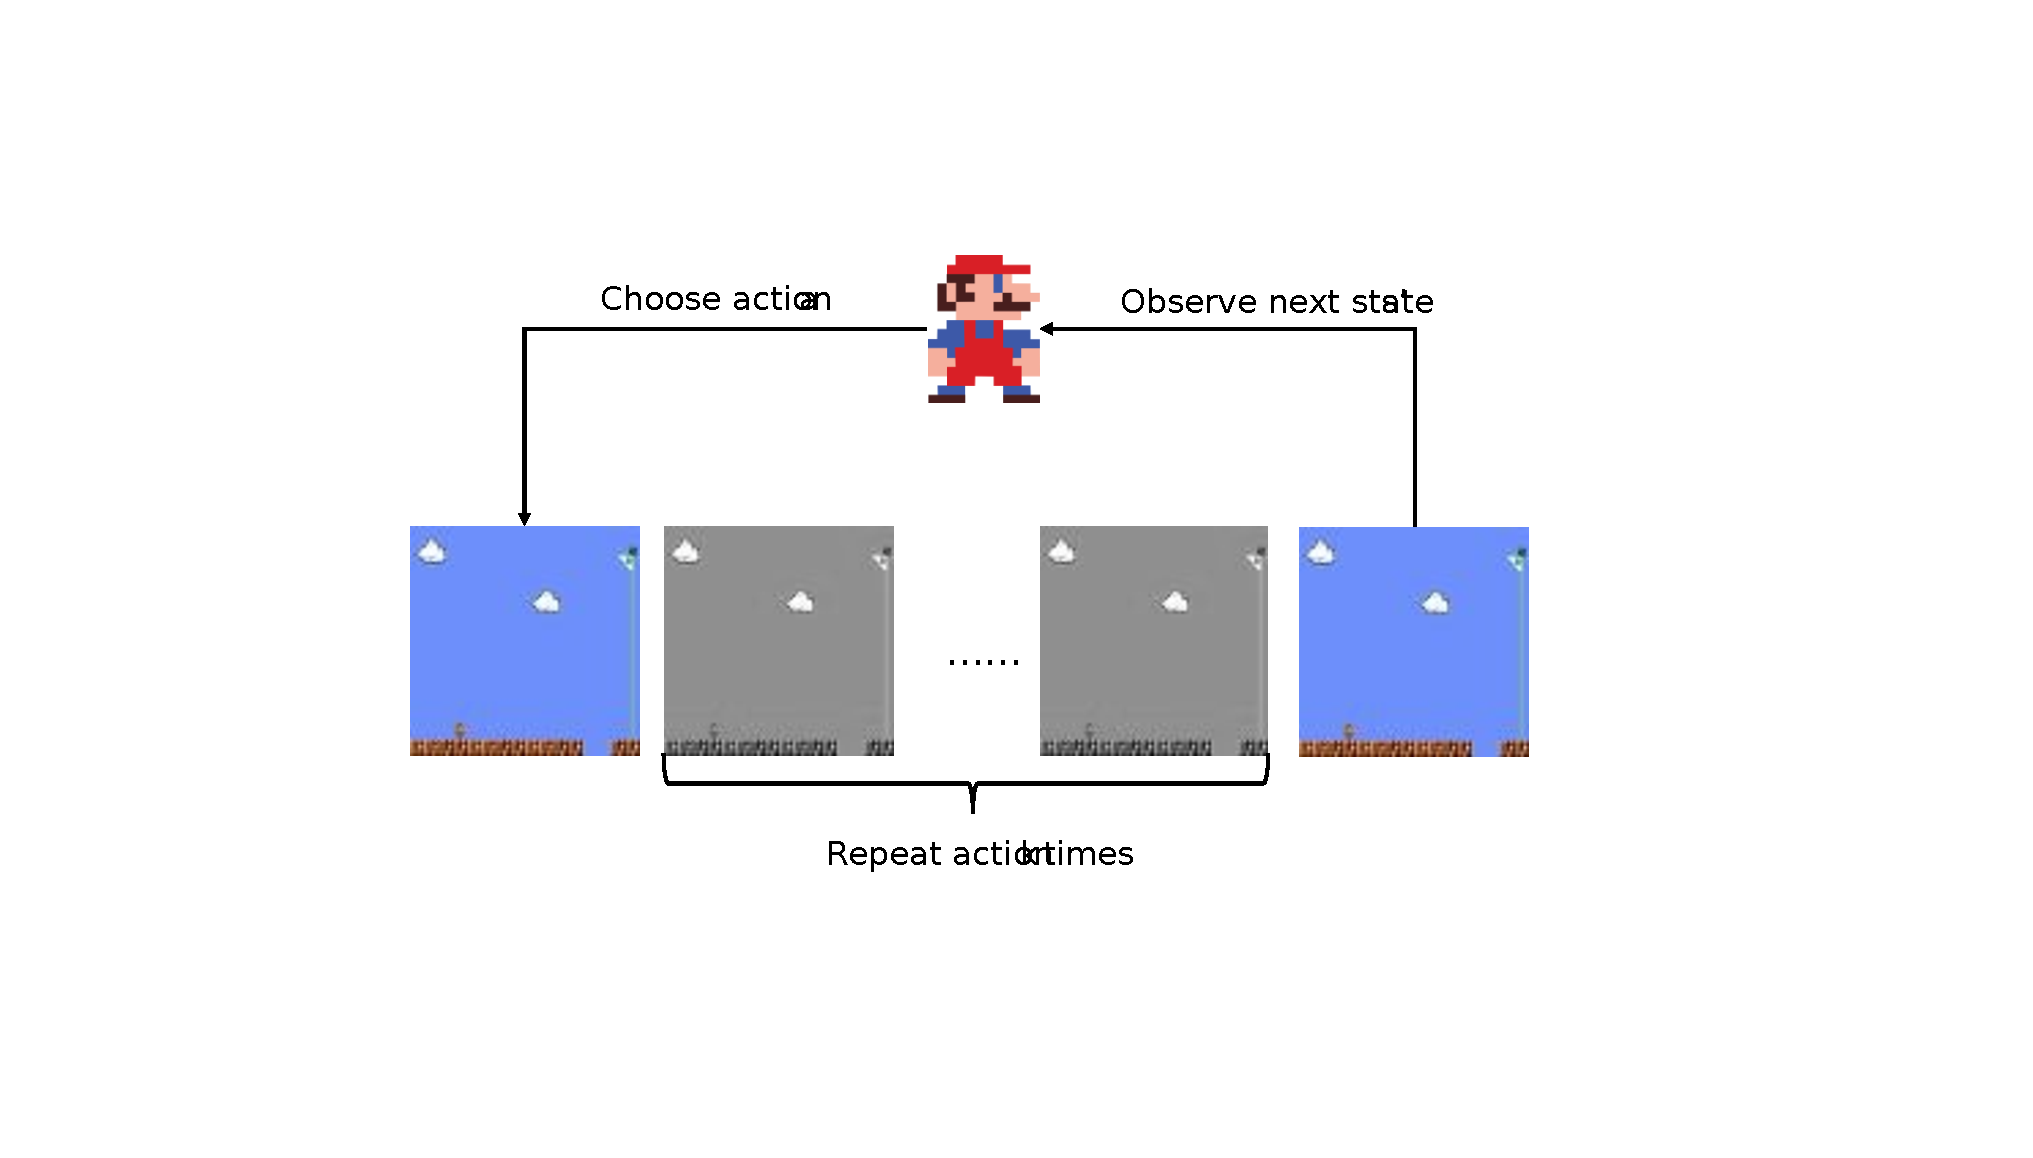
\includegraphics[trim={0 4cm 0 4cm}, clip, width=1\linewidth]{figs/frame_skipping.eps}
\caption{The agent selects action $a$ to be executed $k$ times in the emulator and observes the $k^{th}$ frame}.
\end{figure}

\subsection{Custom Levels}\label{custom_levels}
Investigating whether agents can learn skills and reuse is best done with custom levels. A custom level represents a skill the agent ought to learn and therefore provides a closed off space where learning can take place. The project used three custom built levels - two where agents were meant to learn a basic skill, as well as a third one which is a combination of the two basic levels. Regardless of the skill that agents are supposed to learn, the goal is still to reach the flag at the end. In the system, levels are \texttt{.txt} files with ASCII art and can rapidly be created and changed if needed. The three levels created for this project were:

\begin{enumerate}
	\item \textbf{Steps with Gap}\\
	In this level, the skill to be learned is to jump up the steps and across the gap to reach the flag on the other side.
	
	
	\item \textbf{Two Pipes}\\
	In this level, the agent needs to learn how to jump over pipes. Though it also involves jumping, overcoming a pipe requires a different set of primitive actions than crossing steps with a gap.
	
	\item \textbf{Steps with Gap + Two Pipes}\\
	A combination of the previous two levels, the agent needs to overcome pipes as well as steps with a gap in the middle before reaching the flag.
\end{enumerate}


	\begin{figure}[!htb]
\minipage[t]{0.25\textwidth}
  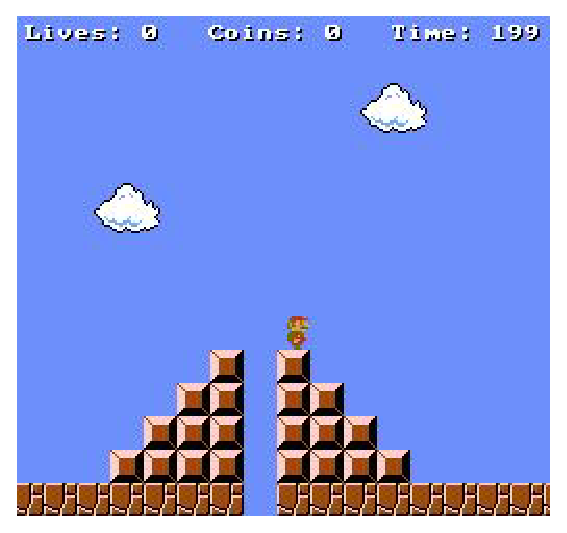
\includegraphics[width=\linewidth]{figs/steps_gap_level.eps}
  \caption{Steps with Gap Level}\label{fig:steps_gap_level}
\endminipage\hfill
\minipage[t]{0.25\textwidth}
  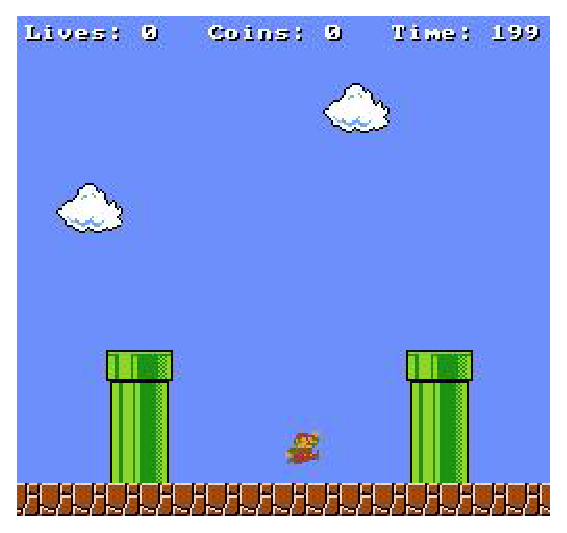
\includegraphics[width=\linewidth]{figs/two_pipe_level.eps}
  \caption{Two Pipes Level}\label{fig:}
\endminipage\hfill
\minipage[t]{0.25\textwidth}%
  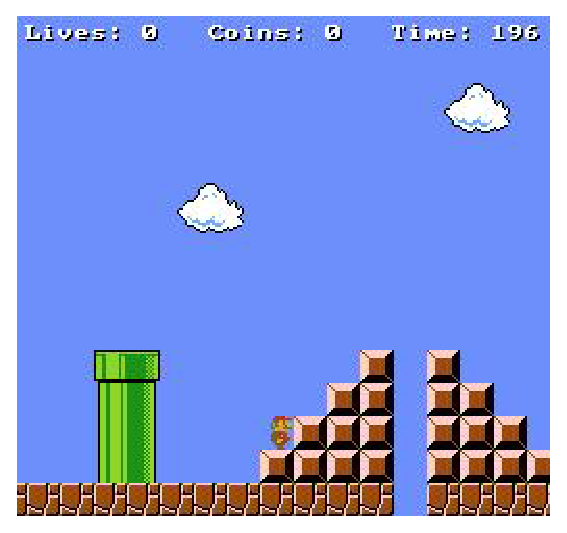
\includegraphics[width=\linewidth]{figs/steps_pipe_level.eps}
  \caption{Steps with Gap + Two Pipes}\label{fig:awesome_image3}
\endminipage
\end{figure}

The project is confined to only teaching Mario navigation tasks, hence why none of the levels include any enemies. The reasoning behind this is the state space associated with dynamic and static objects. Pipes, gaps, and steps are static objects that do not move around in the world. A Goomba or Koopa on the other hand is dynamic and forces Mario to learn more states before knowing how to act around it.



\section{Experiment Design}
The goal of this project is to investigate whether introducing hierarchies, temporal abstraction and sequential learning into RL speeds up the learning process. A good indicator of a model's learning process is how quickly it is able to accumulate rewards. Models that learn quickly, will have discovered actions which return large rewards sooner than slow learning models. Therefore, the main metric used to compare the different RL models will be the average reward per episode. To judge whether learning hierarchies is beneficial to learning speed, the same Mario model is trained sequentially on three levels. The first two levels are designed for Mario learn specific skills - navigating steps and jumping over pipes respectively (section \ref{custom_levels}). The third level is a combination of the two previous levels and requires the previously learned skills to be solved. An agent which has learned reusable hierarchies should in theory adopt to the new environment faster than a flat-learning agent. Adopting in this sense means to acquire rewards faster, which should show in an initially steeper reward curve. To judge whether learning \textit{sequentially} gives a learning advantage, the agents will also be compared against \textit{non-sequential} versions of themselves. These are models which have not been trained on previous levels and come without any prior knowledge. The purpose of this comparison is to investigate whether training agents \textit{sequentially} is beneficial over learning from scratch.

\begin{table}[h!]
\centering
\begin{tabular}{ |c|c|c|c|c|c| } 
 \hline
 \textbf{Model} & \textbf{Level} & \textbf{Sequential} & \textbf{Frames} & \textbf{Runtime}\\
 \hline 
 DQN & Steps with Gap & False & $2 \times 10^5$ & 1d 3h 54m 59s\\ 
 \hline
 DQN & Two Pipes & False & $2 \times 10^5$ & 1d 5h 31m 54s\\ 
 \hline
 DQN & Steps with Gap + Two Pipes & False & $2 \times 10^5$ & 1d 5h 46m 34s \\ 
 \hline
DQN & Two Pipes & True & $2 \times 10^5$ & 1d 6h 58m 31s\\ 
 \hline
 DQN & Steps with Gap + Two Pipes & True & $2 \times 10^5$ & 1d 5h 59m 9s\\ 
 \hline 
 Option Critic & Steps with Gap & False & $2 \times 10^5$ & 1d 8h 33m 34s\\ 
 \hline
 Option Critic & Two Pipes & False & $2 \times 10^5$ & 1d 17h 35m 37s\\ 
 \hline
 Option Critic & Steps with Gap + Two Pipes & False & $2 \times 10^5$ & 1d 9h 32m 13s\\ 
 \hline
Option Critic & Two Pipes & True & $2 \times 10^5$ & 1d 19h 33m 13s\\ 
 \hline
 Option Critic & Steps with Gap + Two Pipes & True & $2 \times 10^5$ & 1d 13h 7m 29s\\ 
 \hline
 
  FuN & Steps with Gap & False & $2 \times 10^5$ & 1d 14h 40m 8s\\ 
 \hline
 FuN & Two Pipes & False & $2 \times 10^5$ & 1d 13h 58m 52s\\ 
 \hline
 FuN & Steps with Gap + Two Pipes & False & $2 \times 10^5$ & 1d 12h 13m 18s\\ 
 \hline
FuN & Two Pipes & True & $2 \times 10^5$ & 1d 17h 14m 25s\\ 
 \hline
 FuN & Steps with Gap + Two Pipes & True & $2 \times 10^5$ & 1d 14h 4m 24s\\ 
 \hline
 
\end{tabular}
\caption{Experiments carried out for the project. sequential indicates whether the model has been pretrained on another level already.}
\label{tbl:experiments}
\end{table}

Determining the stopping criterion for the experiments, i.e. when the model should stop learning, was grounds to some experimentation. Letting agents play a set number of episodes is common, however episodes vary in length across different levels as well as in the same level. This variation means that agents will have had different amount of playtime as better agents would finish sooner. Therefore, there would be no guarantee that agents get the same number of experiences. It was decided to let all agents experience the same number of frames of the game to better predict training times and to also use the number of completed episodes as an indicator of performance. A fast-learning agent should be able to play through more episodes using the same number of timesteps than a slow-learning agent. Thus, the completed number of episodes after $t$ timesteps can also be used to compare the different RL models. While it is desirable to run experiments multiple times to ensure that the observations do not represent noise, financial limitations and long training times only allowed a single run per experiment. 



\section{Results}

\subsection{DQN Agent}\label{dqn_experiment}
%Using a DQN as a comparison baseline is common in the RL literature \cite{bacon2017option, kulkarni2016hierarchical, hessel2018rainbow, levy2017learning}, thus this project will follow the trend. 
This section will show how the Deep RL theory from section \ref{deep_rl} was used to construct a DQN agent and compare the average reward per episode for sequential and non-sequential models. Additionally, the rewards each agent obtained in the final episode as well as total rewards accumulated over an experiment will be looked at. The DQN agent uses a policy and target network, both of which are CNNs with three convolutional layers followed by two linear layers. The activation function used between the layers is a Rectified Linear Unit (ReLu) \cite{lecun2015deep}, which over the past years established itself as the most popular activation function for training neural networks \cite{ramachandran2017searching}. The agent also has an experience replay buffer of size 100,000. 

\begin{figure}[!htb]
\vspace{-10pt}
\centering
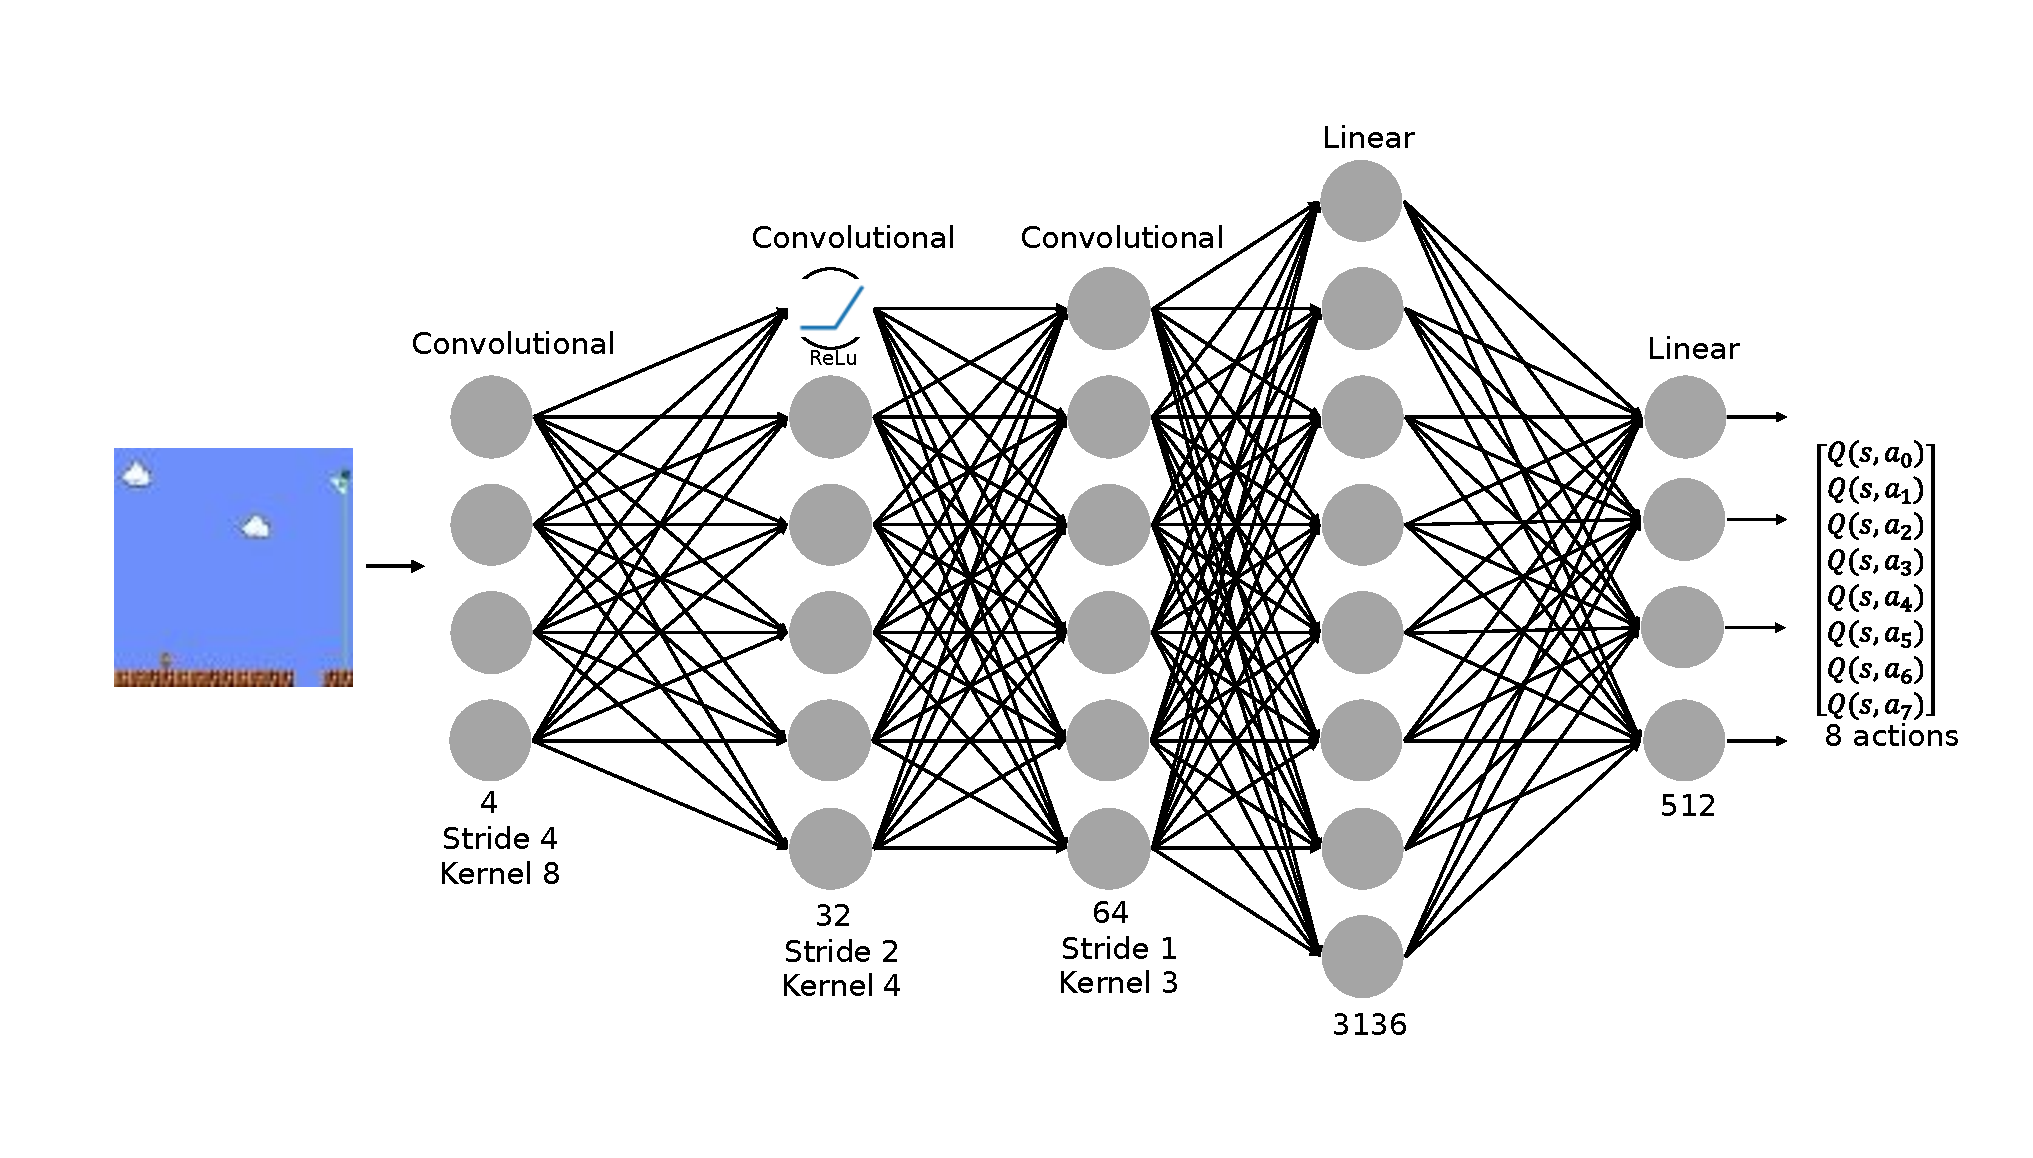
\includegraphics[trim={0 0 0 0}, clip, width=.75\linewidth]{figs/dqn.eps}
\vspace{-20pt}
\caption{Illustration of the CNN used by the DQN Agent (not to scale). Stride is the number of pixels the convolutional filter moves. Kernel is the size of the filter.}
\label{fig:dqn_cnn}
\end{figure}

Choosing the hyperparameters for a model is an important aspect. Performing a grid search \cite{bergstra2012random} for optimising parameters would have been too costly considering the time it took to run each experiment. Therefore, the chosen parameters values were taken from popular RL literature as well as famous DQN implementations.


\begin{table}
	\begin{tabular}{ |c|c|c|c|c|c|c|}
	\hline
	\textbf{$\alpha$} & \textbf{Batch Size} & \textbf{$\gamma$} & \textbf{Buffer Size} & \textbf{Target Update Freq} & \textbf{Learn Freq} & \textbf{Learn Start}\\
	\hline
	0.0001 & 32 & 0.99 & 100,000 & 200 & 4 & 50,000 \\
	\hline
	\end{tabular}
	\captionsetup{singlelinecheck=off}
	\caption[DQN Hyperparameters]{DQN Hyperparameters where: \begin{itemize}
	\itemsep0em 
		\item \textbf{$\alpha$}: Learning Rate.
		\item \textbf{Batch Size}: The number of samples used to train the network each training epoch.
		\item \textbf{$\gamma$}: Discount Factor.
		\item \textbf{Buffer Size}: Size of the replay buffer.
		\item \textbf{Target Update Freq}: Frequency in timesteps the weights from the policy net are copied to the target net.
		\item \textbf{Learn Freq}: Frequency in timesteps the network is trained, e.g. every 4th frame.
		\item \textbf{Learn Start}: When the agent should start sampling from the replay memory and train the network.
	\end{itemize}}
	\label{tbl:dqn_hyperparams}
\end{table}


\begin{figure}[t]
     \centering
     \begin{subfigure}[t]{0.32\textwidth}
         \centering
         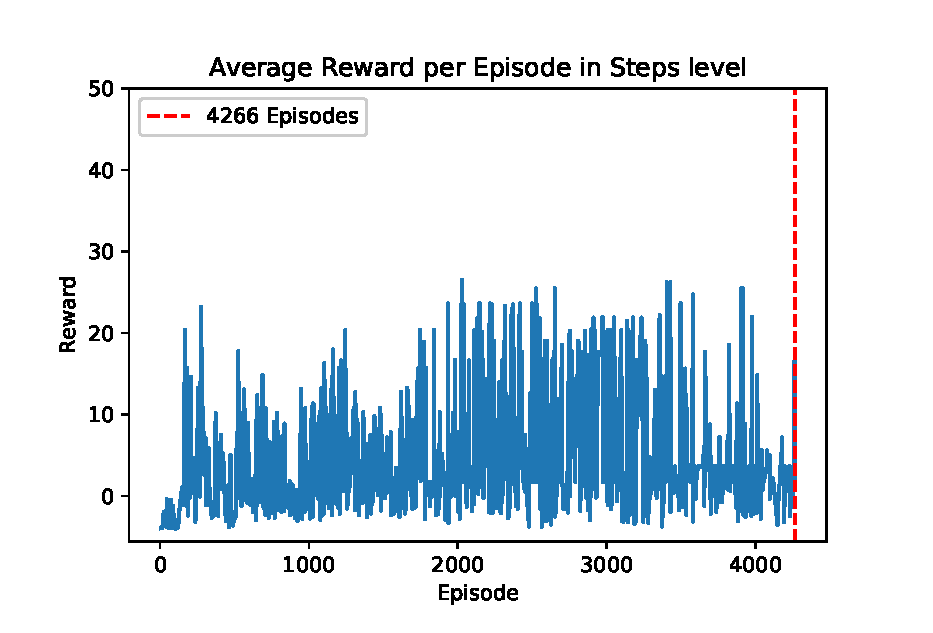
\includegraphics[width=\textwidth]{figs/dqn_results_1.eps}
         \caption{}
         \label{fig:dqn_results_1}
     \end{subfigure}
     \hfill
     \begin{subfigure}[t]{0.32\textwidth}
         \centering
         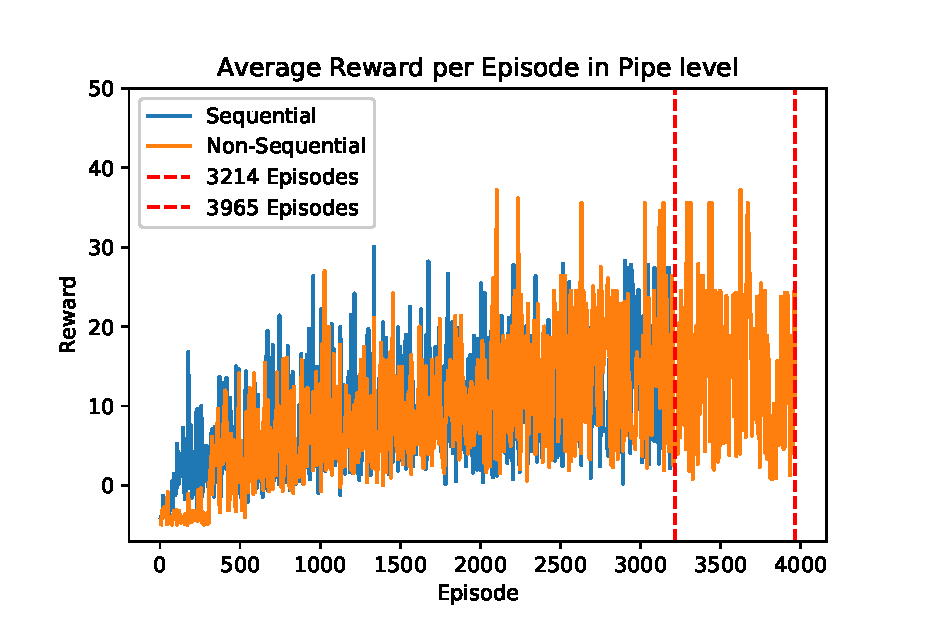
\includegraphics[width=\textwidth]{figs/dqn_results_2.eps}
         \caption{}
         \label{fig:dqn_results_2}
     \end{subfigure}
     \hfill
     \begin{subfigure}[t]{0.32\textwidth}
         \centering
         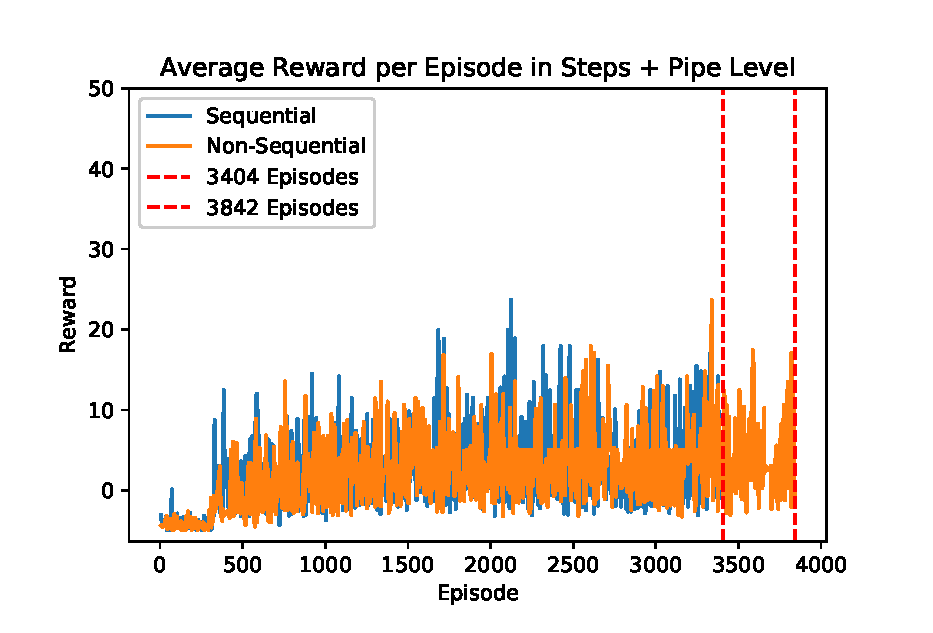
\includegraphics[width=\textwidth]{figs/dqn_results_3.eps}
         \caption{}
         \label{fig:dqn_results_3}
     \end{subfigure}
        \caption{DQN Performance on the three Super Mario levels measured in the average reward per played episode.}
        \label{fig:dqn_results}
\end{figure}

\begin{table}[h!]
\centering
\begin{tabular}{ |c|c|c|c|c|c| } 
	\hline
	\textbf{Levels} & Steps & Sequential Pipe & Pipe & Steps + Pipe & Sequential Steps + Pipe\\
	\hline
	\textbf{Final Rewards} & 128.73 & 225.76 & 322.24 & -25.0 & 242.34 \\
	\hline
	\textbf{Total Rewards} & 409.92 & 2485.56 & 4483.92 & -228.09 & 388.12 \\
	\hline
\end{tabular}
\caption{Rewards accumulated by the DQN agent in each level. Final rewards are the total rewards acquired in the final episode of the run. Total rewards is the sum of all rewards of the run.}
\end{table}

The DQN agent was able to mostly find successful policies for all three levels, accumulating mostly positive rewards in all except the non-sequential Steps + Pipe level. A successful policy should lead to a net positive reward for the agent in the very last episode of the run. In the last episode, the agent is fully exploiting the environment by only choosing optimal actions. Hence, if the agent has learned a successful policy, it is expected that the total reward in the last episode is positive. The results also show that a sequential agent who has been trained on the steps level is able to accumulate rewards faster at first in the pipe level when compared to an agent who has to learn the level from scratch (see the first 250 episodes in \ref{fig:dqn_results_2}). Thereafter, the two models have nearly identical reward curves however. The non-sequential agent manages to accumulate a higher reward in the final episode of the run in the pipe level, suggesting that the model learned a better policy. Looking at the total rewards per run, it can be confirmed that the non-sequential model accumulated more in total as well. In the final level where the steps and pipes were combined to test Mario's abilities to reuse information (\ref{fig:dqn_results_3}), both the sequential and non-sequential model learned at about equal speeds. Although here the sequential model appears to have found a more successful policy as it has more rewards in the final episode as well as over the entire run. To sum up, the sequentially trained agent enjoys an initial advantage over the non-sequential agent after having been trained on a previous level. The data does not show whether the sequential models find better policies overall however.


\subsection{Option-Critic Agent}\label{oc_experiment}
The Option Critic implementation follows that of a DQN with the addition of the options framework on top. It is an added layer of complexity, which shows in the experiment runtimes - learning the additional subpolicies takes extra time. Option Critic uses a CNN with the same structure as the DQN (see \ref{fig:dqn_cnn}) to learn policies and utilises a policy and target network to avoid overestimating Q-values. Additionally, it also uses the concept of experience replay with a replay buffer of size 100,000 to store observation tuples in and utilises the DQN values for the rest of the hyperparameters as well (see \ref{tbl:dqn_hyperparams}). Lastly, the number of options to be learned was specified at 2, taking after the authors of the Option Critic paper \cite{bacon2017option}. The code was sourced from public github repositories \cite{oc_github} and adapted to fit the specifications of the project.


\begin{figure}[htb!]
     \centering
     \begin{subfigure}[t]{0.32\textwidth}
         \centering
         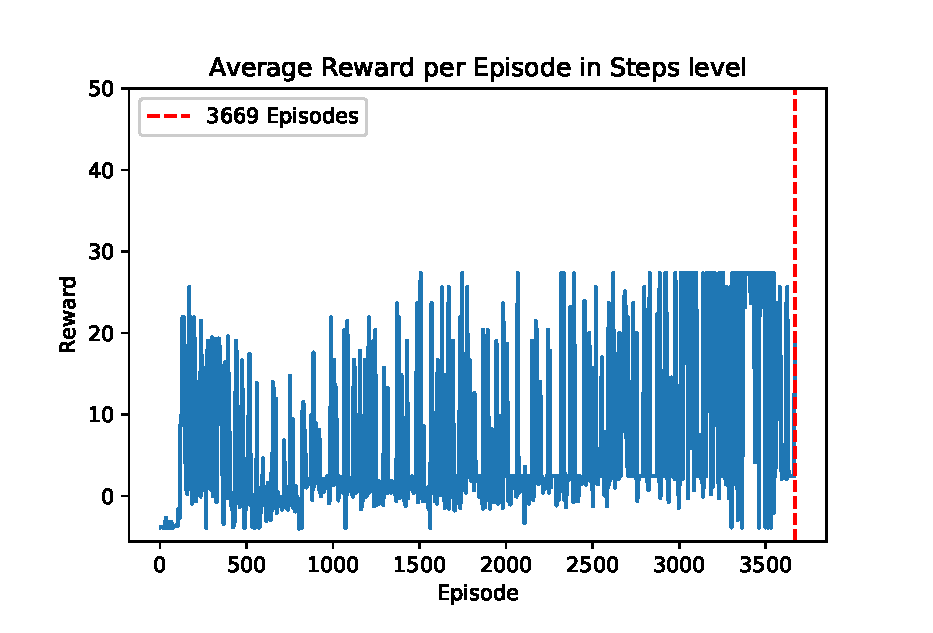
\includegraphics[width=\textwidth]{figs/oc_results_1.eps}
         \caption{}
         \label{fig:oc_results_1}
     \end{subfigure}
     \hfill
     \begin{subfigure}[t]{0.32\textwidth}
         \centering
         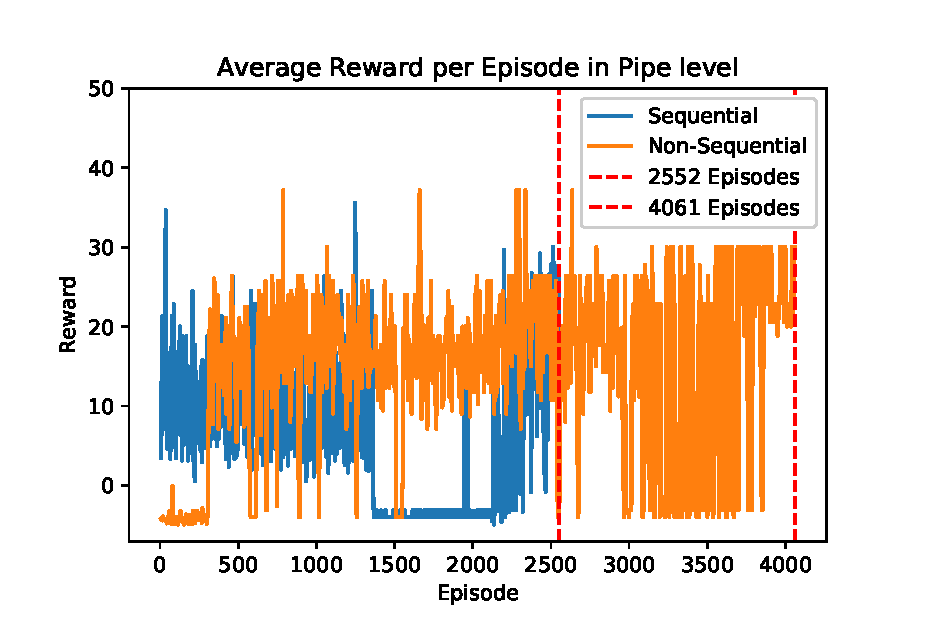
\includegraphics[width=\textwidth]{figs/oc_results_2.eps}
         \caption{}
         \label{fig:oc_results_2}
     \end{subfigure}
     \hfill
     \begin{subfigure}[t]{0.32\textwidth}
         \centering
         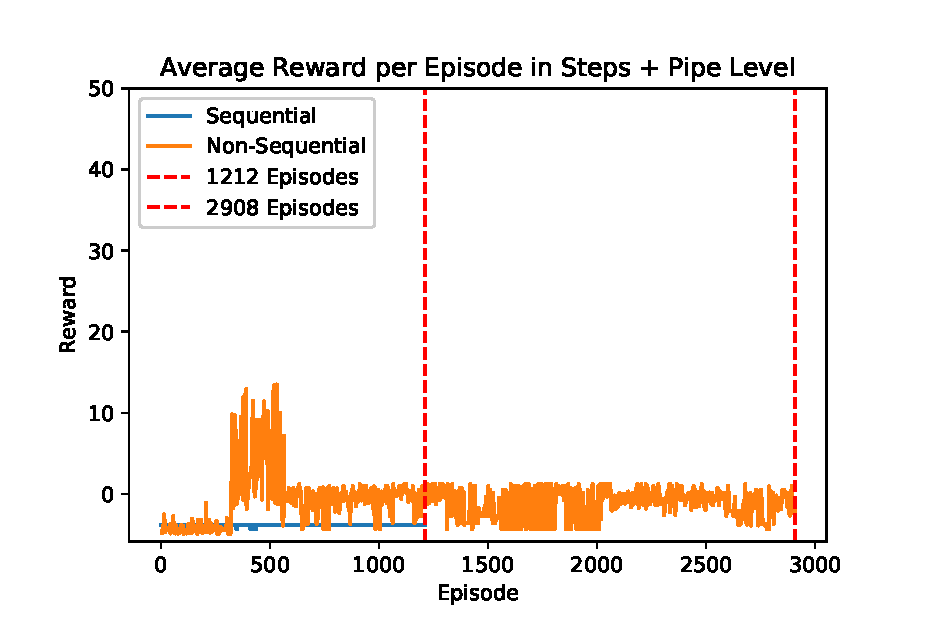
\includegraphics[width=\textwidth]{figs/oc_results_3.eps}
         \caption{}
         \label{fig:oc_results_3}
     \end{subfigure}
        \caption{Option Critic Performance on the three Super Mario levels measured in the average reward per played episode.}
        \label{fig:oc_results}
\end{figure}

\begin{table}[htb!]
\centering
\begin{tabular}{ |c|c|c|c|c|c| } 
	\hline
	\textbf{Levels} & Steps & sequential Pipe  & Pipe & Steps + Pipe & sequential Steps + Pipe \\
	\hline
	\textbf{Final Rewards} & 342.47 & 336.71 & 420.62 & -309.0 & -629.0\\
	\hline
	\textbf{Total Rewards} & -471.95 & 186.54 & 4492.79 &  -2687.05 & -3870.95 \\
	\hline
\end{tabular}
\caption{The total sum of credits accumulated in each level by the Option Critic agent.}
\label{tbl:oc_rewards}
\end{table}

Overall, the performance of the Option Critic is very erratic and unstable in all levels. The average reward obtained per episode goes through extreme fluctuations from values just below zero up to values of thirty. As the episode count goes up the agent is meant to slowly converge on a master policy which returns more rewards than a policy earlier in the run. Though Option Critic agent appears to only be showing minimal improvement over the duration of a run, its final policies actually outperform the DQN on the Steps, sequential Pipe, and Pipe runs (see Final Rewards in Table \ref{tbl:oc_rewards}). Like the DQN, the results show that a sequential agent who has been trained on a previous level is to quicker to adapt to the new environment (see the first 250 episodes in \ref{fig:oc_results_2}). Adapting quickly means to require fewer episodes to finding actions which return larger rewards. However, the non-sequential model outperforms the sequential model in the late stages of the run for both the Pipe and Steps + Pipe levels (see final and total rewards in Table \ref{tbl:oc_rewards}). Occasionally, the Option Critic gets stuck in local minima which can be seen as the flat sections with low reward values in the reward curve (see sequential \ref{fig:oc_results_2} and sequential \ref{fig:oc_results_3}). It indicates that Mario has gotten stuck somewhere in the level and keeps accumulating the negative reward for letting the time pass. The agent manages to leave the local minimum in the Pipe level but not in the Steps + Pipe level. To summarise, the sequential model outperforms the non-sequential model in the early stages of the Steps level however finds an overall worse policy. The data also suggests that the non-sequential models find better policies. 


%Why OC failed?
%* not enough options
%* only tested on a simple domains

\subsection{FuN Agent}\label{fun_experiment}
The implementation of the FuN agent differs from that of the DQN and Option Critic. Though it also has a CNN with ReLu activation functions, the number of layers as well as values for stride and kernel are different. This is because the CNN does not compute the Q-values but an intermediate state representation that is to be used further down the processing pipeline. Because FuN uses recurrent networks in the form of LSTMs to compute an action distribution for the agent, the architecture requires neither memory replay nor target networks. Hence, FuN has a lower memory footprint than both the DQN and Option Critic which might have to store millions of experiences for more complex problems. The intricate design of the FuN agent is more computationally expensive however as can be seen in the experiment runtimes (see Table \ref{tbl:experiments}). As with the Option Critic and DQN agent, the code for the FuN agent was taken from a public github repository \cite{fun_github} and altered to fit the project specifications.

\begin{figure}[htb!]
     \centering
     \begin{subfigure}[t]{0.32\textwidth}
         \centering
         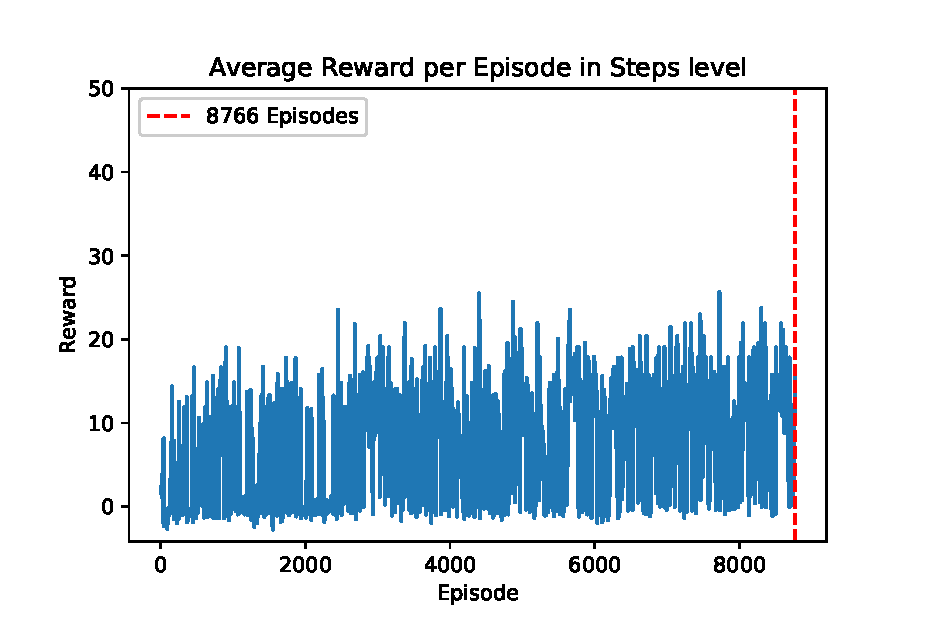
\includegraphics[width=\textwidth]{figs/fun_results_1.eps}
         \caption{}
         \label{fig:fun_results_1}
     \end{subfigure}
     \hfill
     \begin{subfigure}[t]{0.32\textwidth}
         \centering
         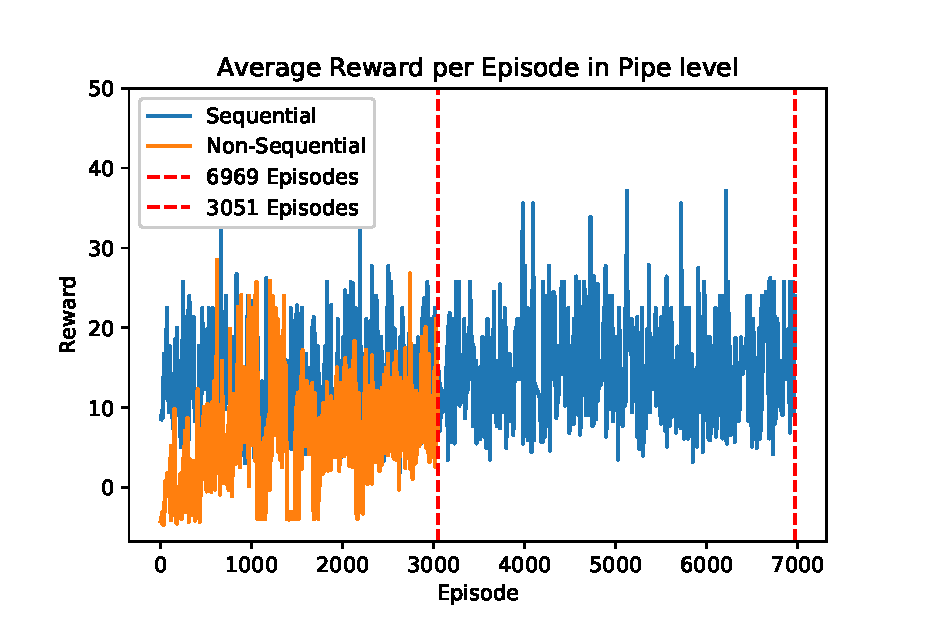
\includegraphics[width=\textwidth]{figs/fun_results_2.eps}
         \caption{}
         \label{fig:fun_results_2}
     \end{subfigure}
     \hfill
     \begin{subfigure}[t]{0.32\textwidth}
         \centering
         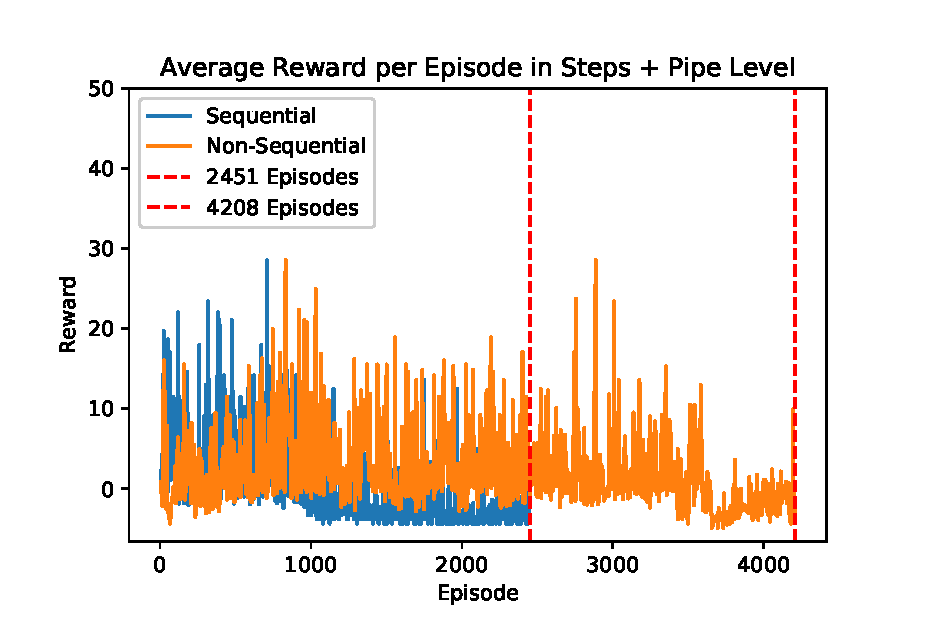
\includegraphics[width=\textwidth]{figs/fun_results_3.eps}
         \caption{}
         \label{fig:fun_results_3}
     \end{subfigure}
        \caption{FuN Performance on the three Super Mario levels measured in the average reward per played episode.}
        \label{fig:fun_results}
        
\end{figure}

\begin{table}[htb!]
\centering
\begin{tabular}{ |c|c|c|c|c|c| } 
	\hline
	\textbf{Levels} & Steps & Sequential Pipe  & Pipe & Steps + Pipe & Sequential Steps + Pipe \\
	\hline
	\textbf{Final Reward} & 330.47 & 408.62 & 283.04 & -409.73 & -629.0 \\
	\hline
	\textbf{Total Rewards} & 6595.49 & 11032.36 & 2166.36 & 694.201 & -2541.22 \\
	\hline
\end{tabular}
\caption{Total rewards accumulated by the FuN agent in the final episode of the run and in the overall run.}


\end{table}

Out of the three agents, the FuN agent was able to accumulate the most total rewards in the Steps, sequential Pipe and Steps + Pipe level. It also outperformed the DQN on the final rewards in the Steps and the sequential Pipe level. As with the DQN and Option Critic, the sequential model which was trained on the Steps level outperforms that of a model which learns the level from scratch (see the first 1000 episodes in \ref{fig:fun_results_2}). Whereas the sequential DQN and Option Critic models were outperformed by the non-sequential counterparts later in the run, the sequential FuN does better than the non-sequential FuN in the final reward and total reward. Much like the the Option Critic, FuN has a worse performance than the DQN on the final Steps + Pipe level. Here, both the sequential and non-sequential FuN perform similarly in the beginning. The sequential model converges to a suboptimal policy as it keeps accumulating negative rewards. In summary, the sequential model outperforms its non-sequential counterpart throughout of the Steps level. This is a contrasting experience to the DQN and Option Critic where the sequential model started strong but found an overall worse policy. For this reason, it is less clear whether sequential models also find better policies than non-sequential models.

\subsection{Evaluation of Results}
Comparing the sequential models against non-sequential models showed that sequential models have an initial advantage over non-sequential models when being placed in a new environment. They accumulate rewards quicker in the beginning because the weights of the policy network have already been trained on a somewhat related environment. Thus, the models becomes equipped with previous knowledge they can use to their favour. The next step is to compare how the various sequential models perform when being placed in a novel environment. A flat learning agent like the DQN should accumulate knowledge of lower quality than the the hierarchical agents because it does not have temporally abstract actions available. Quality of knowledge in this case is measured by its reusability. Knowledge which can be transferred to new spaces is highly reusable and of high quality. Likewise, knowledge which is only applicable to a narrow space is of poor reusability and thus low quality. The Option Critic and FuN agent are expected to learn reusable subpolicies which should translate to higher quality knowledge and therefore more rewards in the novel environment. 

\begin{figure}[htb!]
     \centering
     \begin{subfigure}[t]{0.48\textwidth}
         \centering
         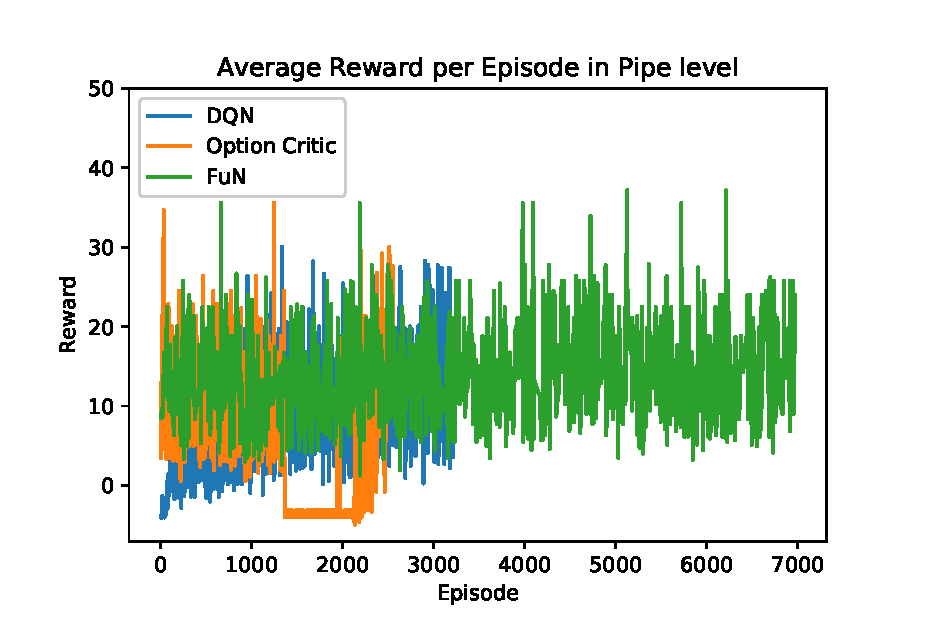
\includegraphics[width=\textwidth]{figs/all_results_1.eps}
         \caption{}
         \label{fig:all_results_1}
     \end{subfigure}
     \hfill
     \begin{subfigure}[t]{0.48\textwidth}
         \centering
         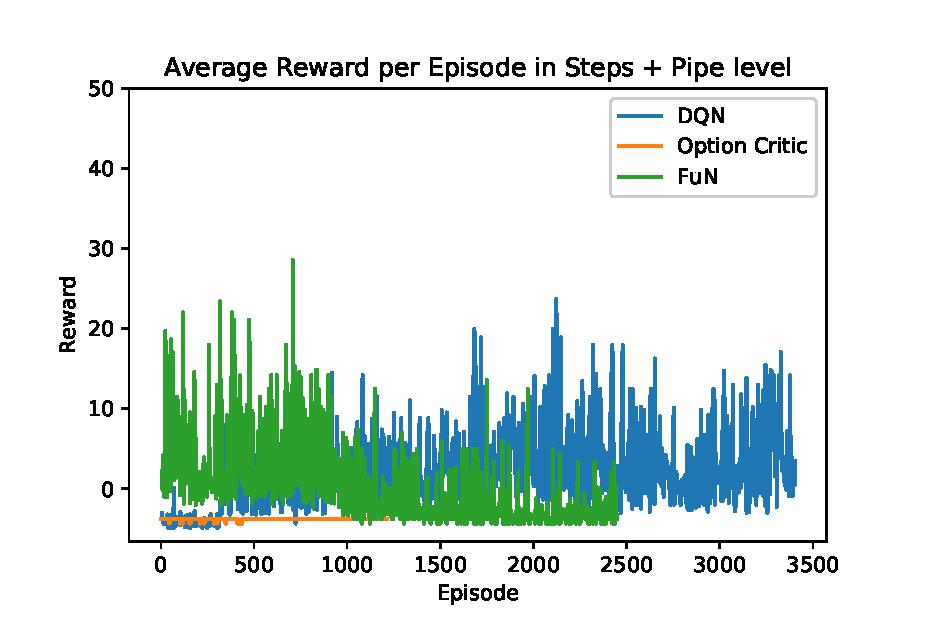
\includegraphics[width=\textwidth]{figs/all_results_2.eps}
         \caption{}
         \label{fig:fun_results_2}
     \end{subfigure}
     \hfill
        \caption{Comparing the average rewards per episode for the two levels where models were pretrained.}
        \label{fig:all_results}
       
\end{figure}

Comparing the average rewards per episode for all three sequentially trained algorithms shows that the hierarchical models have an initial advantage over the DQN in the Pipe level. Both the FuN and Option Critic agent are able to obtain higher rewards than the DQN in the first 1,000 episodes of the run. This suggests that they learned reusable hierarchies in the Steps level they were previously trained on. Additionally, the learned hierarchies are superior to the learning achievements of the DQN because they allowed the agents to choose actions which lead to higher rewards. Though the DQN catches up with the hierarchical models later, initially it cannot capitalise on the information from the previous Steps level as much as hierarchical models. The same cannot be said for the the final Steps + Pipe level however as it gives inconclusive results on whether hierarchical models can exploit previously learned knowledge. The FuN agent initially obtains high rewards but converges to a suboptimal policy. The Option Critic is stuck in a suboptimal policy from the start and the DQN starts out with low rewards but is able to find a successful policy in the end. Training pre-trained models on new environments may cause them to forget what they previously learned because they overwrite their knowledge. This would explain the inconsistent results for the performance of sequential models compared against non-sequential models for the average rewards per episode for the Steps + Pipe level in the previous sections (\ref{dqn_experiment}, \ref{oc_experiment}, \ref{fun_experiment}). Whereas the sequential FuN model learned quicker than its counterpart, the opposite was true for the Option Critic. The DQNs learned at around the same speed. Therefore, it can only be concluded that hierarchical sequential models have an initial learning advantage going from the Steps to the Pipe level. Adding another level to the sequence appears to cause something known as \textit{catastrophic forgetting}. When neural networks are continuously learning new tasks, the weights that were used to solve task A are overwritten to meet the objective of task B \cite{kirkpatrick2017overcoming}. When the network is given task A after learning task B, it has "forgotten" how to solve it. Having learned how to navigate steps and pipes in the first two levels, the various agents fail to reuse the knowledge of the steps level in the final level because the network weights were overwritten in the pipe level.



\subsection{Further Policy Analysis}
%\begin{wrapfigure}{r}{0.5\textwidth}
%\vspace{-40pt}
 % \begin{center}
 %   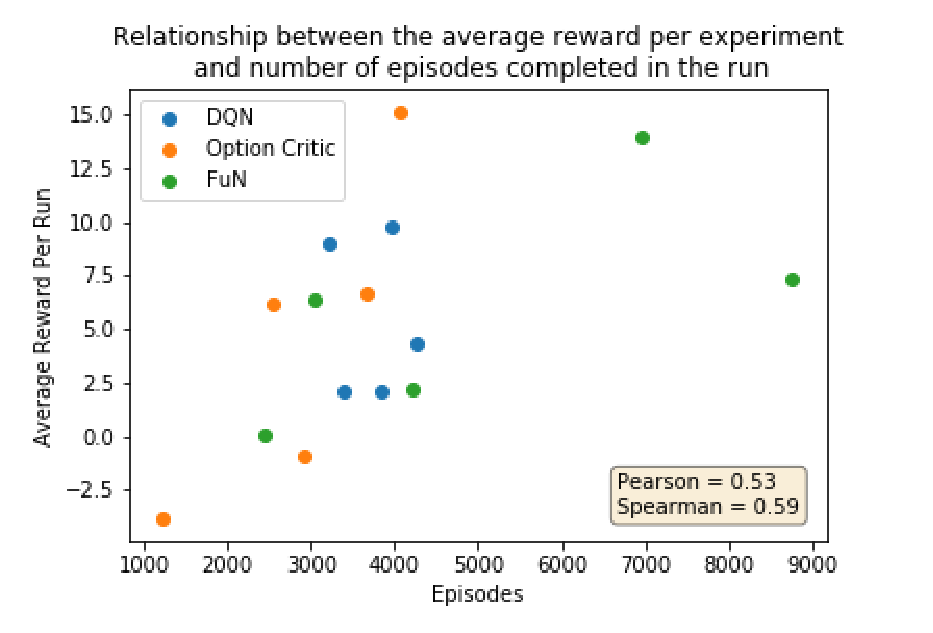
\includegraphics[width=0.48\textwidth]{figs/good_policy.eps}
 % \end{center}
%  \vspace{-20pt}
%  \caption{The average reward per run and the number of completed episodes. Pearson is a linear correlation coefficient. Spearman is a nonlinear correlation coefficient.}
%  \label{fig:good_policy}
%  %\vspace{-40pt}
%\end{wrapfigure}

\begin{figure}[htb!]
	%\vspace{-40pt}
     \centering
     \begin{subfigure}{0.48\textwidth}
         \centering
         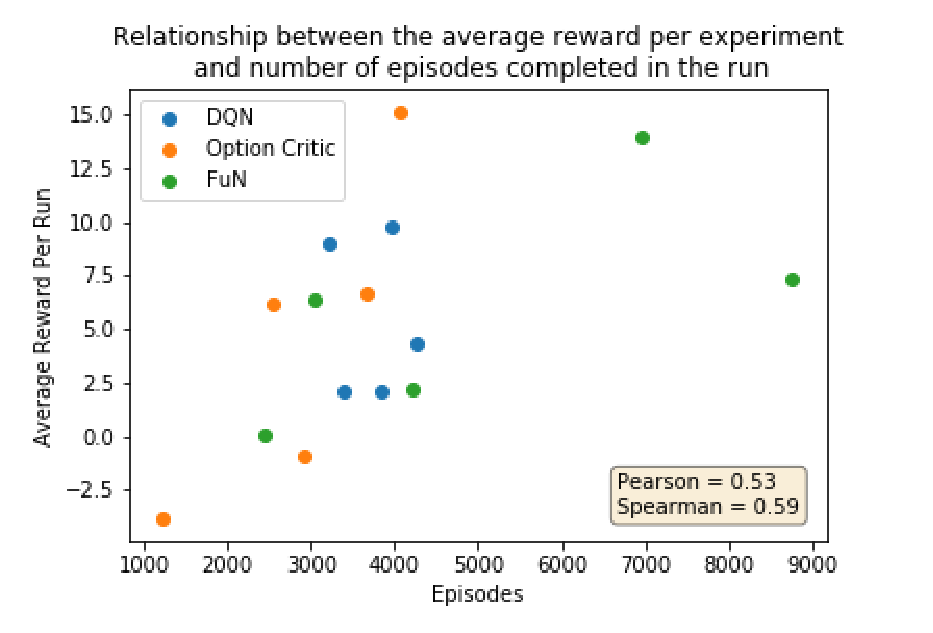
\includegraphics[width=\textwidth]{figs/good_policy.eps}
         \caption{}
         \label{fig:good_policy}
     \end{subfigure}
     \hfill
     \begin{subfigure}{0.48\textwidth}
         \centering
         \includegraphics[width=\textwidth]{figs/sequential_policy_analysis.eps}
         \caption{}
         \label{fig:good_sequential_policy}
     \end{subfigure}
     \hfill
        \caption{The average reward per run and the number of completed episodes. Pearson is a linear correlation coefficient. Spearman is a nonlinear correlation coefficient.}
        \label{fig:all_results}      
\end{figure}

Sequentially trained hierarchical agents are faster learners initially when being shown a new environment (atleast for a task sequence of length 2), but are they able to find better policies? An agent can have a fast learning speed but in the end only find suboptimal policies. An agent who is a fast learner will achieve more rewards faster and play more episodes in the same amount of frames. Using the number of completed episodes shows that the non sequential models for the most part were able to play more episodes than their non-sequential counterparts (see Figure \ref{fig:good_sequential_policy}). However, only relying on the number of completed episodes is not a reliable indicator of a good policy. Playing more episodes does not necessarily correlate with finding a better policy, it just means that you are able to finish an episode faster. An agent acting according to a policy which forces them to commit suicide immediately is able to play many episodes, but will accumulate low rewards. Therefore, looking at the number of completed episodes as the only variable variable will give the illusion of a good policy. Only where the number of completed episodes correlates positively with an overall higher reward can it be concluded that the policy is superior. Figure \ref{fig:good_policy} shows a moderate positive correlation between the number of episodes completed by an agent and the averaged average reward per episode per run. Broadly speaking, the higher the number of episodes completed, the higher the average reward. Thus, an agent that plays more episodes generally ends up with a good policy too. Although, it cannot be concluded that the hierarchical models were able to find better policies than the DQN as figure \ref{fig:good_policy} shows no discernible pattern for the different algorithms. Similarly, the sequential vs non-sequential comparison in 19b only shows that the sequential models found somewhat better policies. The reason behind this might be that the previous knowledge introduces a bias which is initially beneficial but does not benefit the agent in the long term. 

\section{Deviations From Original Specifications}
The project adhered to the original specifications with two exceptions. First, communication between the RL agents and game emulator was supposed to happen with JSON using HTTP requests. After trialling this method it was deemed to slow and exchanged for the faster Py4J bridge. Second, the set of hierarchical algorithms to be tested included the original Options framework and an approach called Multiplicative Compositional Policies (MCP). The Options framework was substituted for the Option Critic model which is a more recent extension of it and was therefore deemed more reflective of the contemporary RL literature. The MCP was exchanged for DeepMind's Feudal Network because of the lack of information and code available, both of which spoke in DeepMind's favour instead.


\section{Critical Assessment of Project}
This section will assess various areas of the project to see whether any changes or expansions could have benefited the project. Moreover, there are components which if added could have contributed positively.

\begin{itemize}
	\item
	\textbf{Experiment Runtimes}\\
	A big problem with the project was the long runtime of the experiments. The cumulative and average runtime of all experiments was 22 days, 44 minutes, 20 seconds and 1 day, 11 hours, 14 minutes and 57 seconds respectively. As a consequence, each experiment could only be run once which means that very little data could be collected. Averaging the results of multiple runs would have given a more definitive representation of the effect that sequential learning and hierarchical algorithms have on the various agents' learning abilities. With a single run per experiment however, the collected data is less reliable. More experiments could have given answers to questions like why the DQN always outperforms the Option Critic and FuN on the Steps + Pipe level, why the Option Critic tends to get stuck in local optima or if these are just random fluctuations. Additionally, the excessively long runtimes prevented discovering good values for hyperparameters which would have required further experiments. There are a number of reasons why experiments ran slow, some of which are outlined below.
	
	
	
	\item
	\textbf{Emulator Development}\\
	The Java framework used for the emulator did not meet the project requirements right out of the box. It was missing endpoints for the Python agents, classes for extracting the frames from the game as well as preprocessing, calculating the reward, and methods for playing the game in a step by step manner. Although necessary for the success of the project, developing all of these functionalities took away valuable time from running experiments because finishing the emulator was a prerequisite for being able to run the entire system.
	
	\item
	\textbf{Slow Game Emulator Speed}\\
	Choosing the less popular \textit{marioai} Java version over the Python \textit{openaigym} version as a game emulator allowed for the easy creation of custom levels, however came at the cost of decreased emulator speed. First, the communication overhead from the Py4J bridge slowed down the agents because they had to wait for a response to be marshalled back to them. Second, the Java emulator had a ceiling for the maximum number of frames per second (fps). Thus, even with more powerful hardware the agents were constrained to a set speed and learning was slowed down.
	
	%\item
	%\textbf{Short Experiments}\\
%	As a consequence of the slow emulator speed, each experiment only ran for 200,000 frames of the game. RL's sample inefficiency however requires many more frames to be effective. 
	
	\item
	\textbf{Additional Levels}\\
	The experiments showed that sequential hierarchical models are quicker to adopt to a new environments than non-sequential traditional models. To further solidify this notion it would be desirable to train the agents in different levels. This would be to make sure that the difference in performance is not due to the specifically chosen level environment, but the agents themselves.
	
	\item	
	\textbf{Exploration Function}\\
	All agents used a linear function to calculate the exploration value $\epsilon$ (see section \ref{exploit_explore}). In multiple experiments, the Option Critic got stuck in local optima. While it is difficult to pin down the exact reason, trialing a non-linear exploration function such as the sinusoidal function \cite{chuchro2017game} which continously moves between more exploration to more exploitation over the course of an experiment could have produced different results. 
	
	\item
	\textbf{Metric for MDP Distance}\\
	To better assess the knowledge transfer abilities between environments, it would be valuable to know how closely related they are. Figuring out the distance between the two environments makes it possible to assess the learning abilities in a more scientific manner. Agents could be asked to transfer knowledge between levels which are increasingly distant from one another. An agent with good transfer skills would be able to apply knowledge to levels that are further away. Metrics such as the Hausdorff or Kantorovich metric which can be used to measure the distance between MDPs \cite{song2016measuring} could have been implemented to determine the difference between levels in Super Mario and construct levels of varying distance.
	
	%\item
	%\textbf{Egocentric Learning} \\
	%The allocentric state representation for the MDP as an $84 \times 84$ RGB image could have been substituted for a lower-dimensional egocentric view of the game. In allocentric learning, the agent sees the entire environment (screen) whereas an egocentric agent only sees Mario's immediate surroundings. Using an egocentric view of the environment, Mario will only take into account the objects that are close to him when learning \cite{byrne2008principle}. This means that many more of the states in the state space are similar and will therefore invoke a similar response from the agent. The state space reduction means fewer states for the agent to learn and therefore a reduced experiment runtime.
	
	\item
	\textbf{Visualise Options}\\
	An interesting addition which would have helped with the analysis of the various algorithms is the visualisation of the hierarchies learned by the agents. The FuN and Option Critic agents both learned temporally abstract behaviour in the various levels, however just looking at the average reward episode does not tell when and where the agent used that behaviour. Additionally, just because the agent learned hierarchies does not mean that these hierarchies are useful. Therefore, showing which hierarchies the agents learned could have been beneficial in explaining the obtained results.
	
	
\end{itemize}


\section{Conclusion}
The general objective of this project was to create a system capable of training various RL agents on the Super Mario game. Traditional RL algorithms have to learn each problem they face from scratch and struggle to transfer already learned knowledge to new situations. As a result, training times for these agents are exceedingly long. For this reason, the project sought to train RL agents sequentially to build up a knowledge pool and to introduce temporal abstraction into the learning process via hierarchies. In the end, one traditional flat learning agent and two hierarchical agents of varying complexity were built and trained on three different Super Mario levels. The non-sequential set of agents was trained from scratch on each level, whereas the sequential set of agents was trained on the levels with the learned weights from previous levels. The agents were compared on their average reward obtained per episode. In general, when compared to the non-sequential models, the sequential models were able to accumulate rewards quicker in the beginning of levels for a task sequence of two, i.e. when they had been pre-trained on one other level before. The ability to make use of sequential learning appears to break down for a task sequence of three however. Comparing the set of sequential agents against each other showed that the Option Critic and FuN have an initial advantage over the DQN when shown a new environment (for a task sequence of 2), though the DQN catches up with them later. Using the average rewards per experiment and number of episodes completed to measure the quality of a policy, no pattern could be detected for DQN, Option Critic and FuN agents. There was no one RL algorithm which unmistakably outperformed the others. Although the non-sequential models can be said to have found somewhat better policies than the  sequential ones. The biggest problem of the analysis and the project as a whole was the small amount of data that was collected due to the long runtime of the experiments. Hence the conclusions should be subject to scrutiny and be investigated further with more and different experiments. Nonetheless, the data that was obtained and analysed provided interesting insights and serves as an adequate starting point for further research. All in all however, the objectives of investigating sequential training and hierarchical agents were met and the project can be considered a success.

\pagebreak

\bibliographystyle{ieeetran}
\bibliography{references}

\end{document}